\section{Roles}
\label{sec:settings-feature-roles}

A role is a named set of permissions that decides what its holder can see and do. Instead of setting permissions member by member, you prepare the role once and assign it to members, positions or organizational units; when a responsibility changes, you edit the role in one place. Open this page when a new responsibility appears, or when someone sees what is not theirs or cannot find what they need. The page is open to whoever may list roles; opening, creating, editing and deleting a role are each a separate permission.

\begin{rcnote}[Example: Horizon]
Horizon’s system administrator presses ① and creates a role named “Visit coordinator”, then assigns it to the Operations Coordinator position. Its permissions reach Omar Haddad because he holds that position, and do not reach Sarah Al-Khatib.
\end{rcnote}

\begin{figure}[H]
\centering
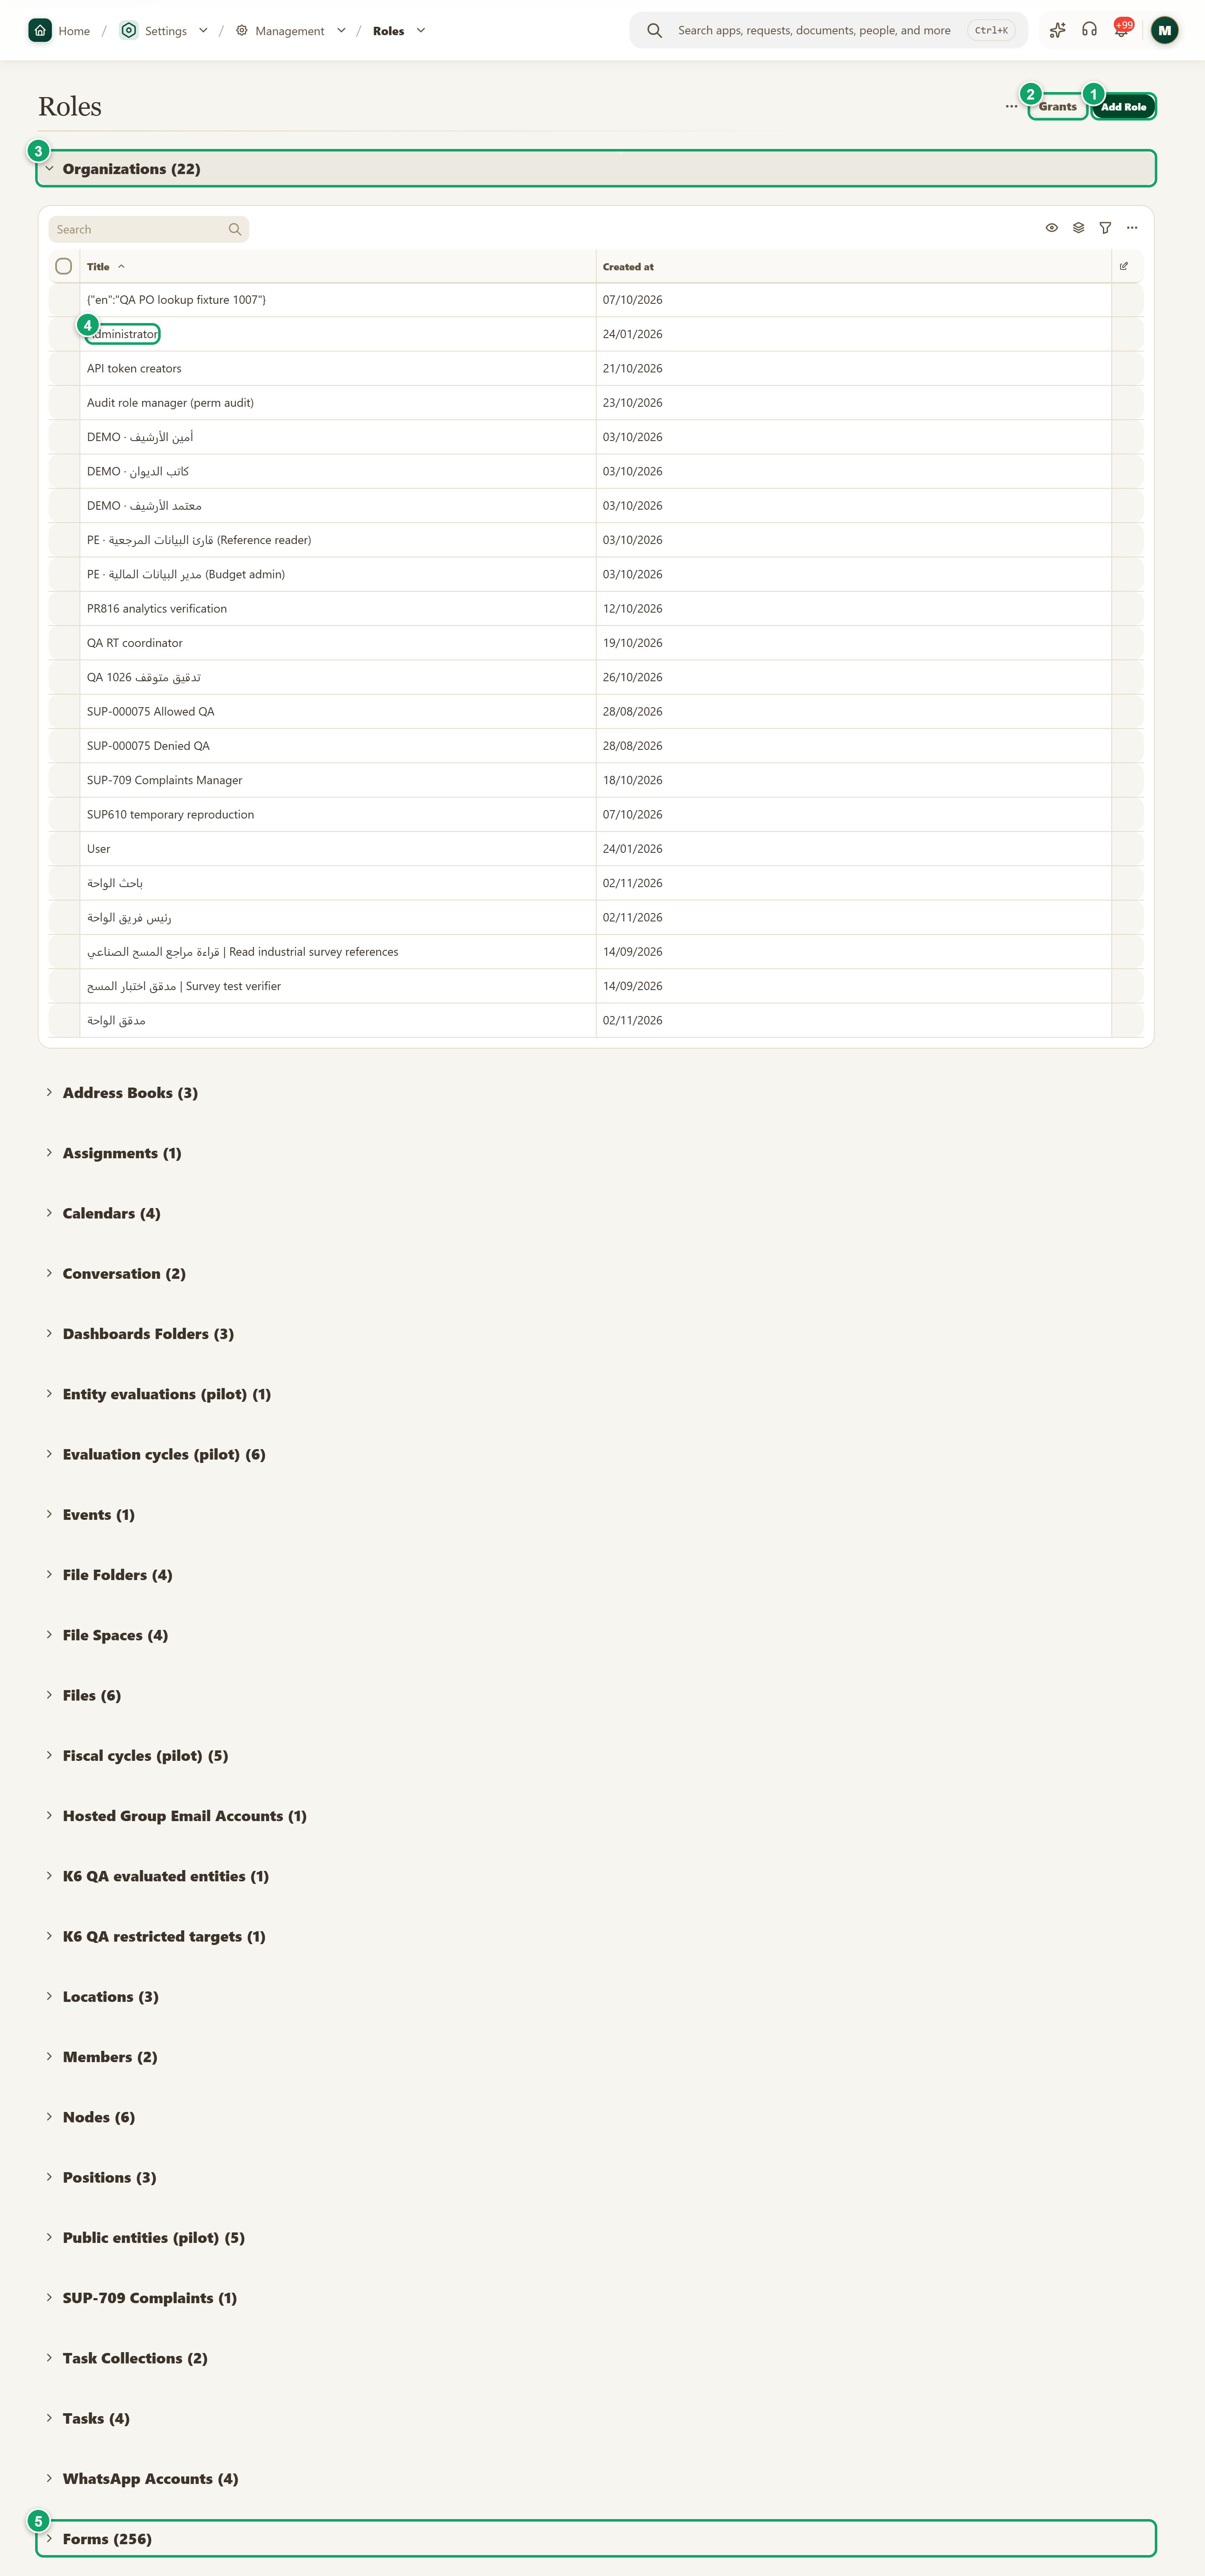
\includegraphics[width=0.95\linewidth,height=0.72\textheight,keepaspectratio]{figures/screens/ch08-roles-en.png}
\caption{The role list, grouped by scope}
\label{fig:settings-roles-screen}
\shotnote{The page lists roles in groups by scope. The scope is where a role’s permissions apply: the whole organization, one record type, or one form. The number beside each group counts its roles; press the group’s name to open it. ① “Add Role”. ② “Grants”: the rules for who may assign roles. ③ The group of roles that apply to the whole organization. ④ A role row: press it to open the role; the row’s menu holds “Duplicate”. ⑤ “Forms”: roles that belong to one form, grouped under its name.}
\end{figure}

\begin{figure}[H]
\centering
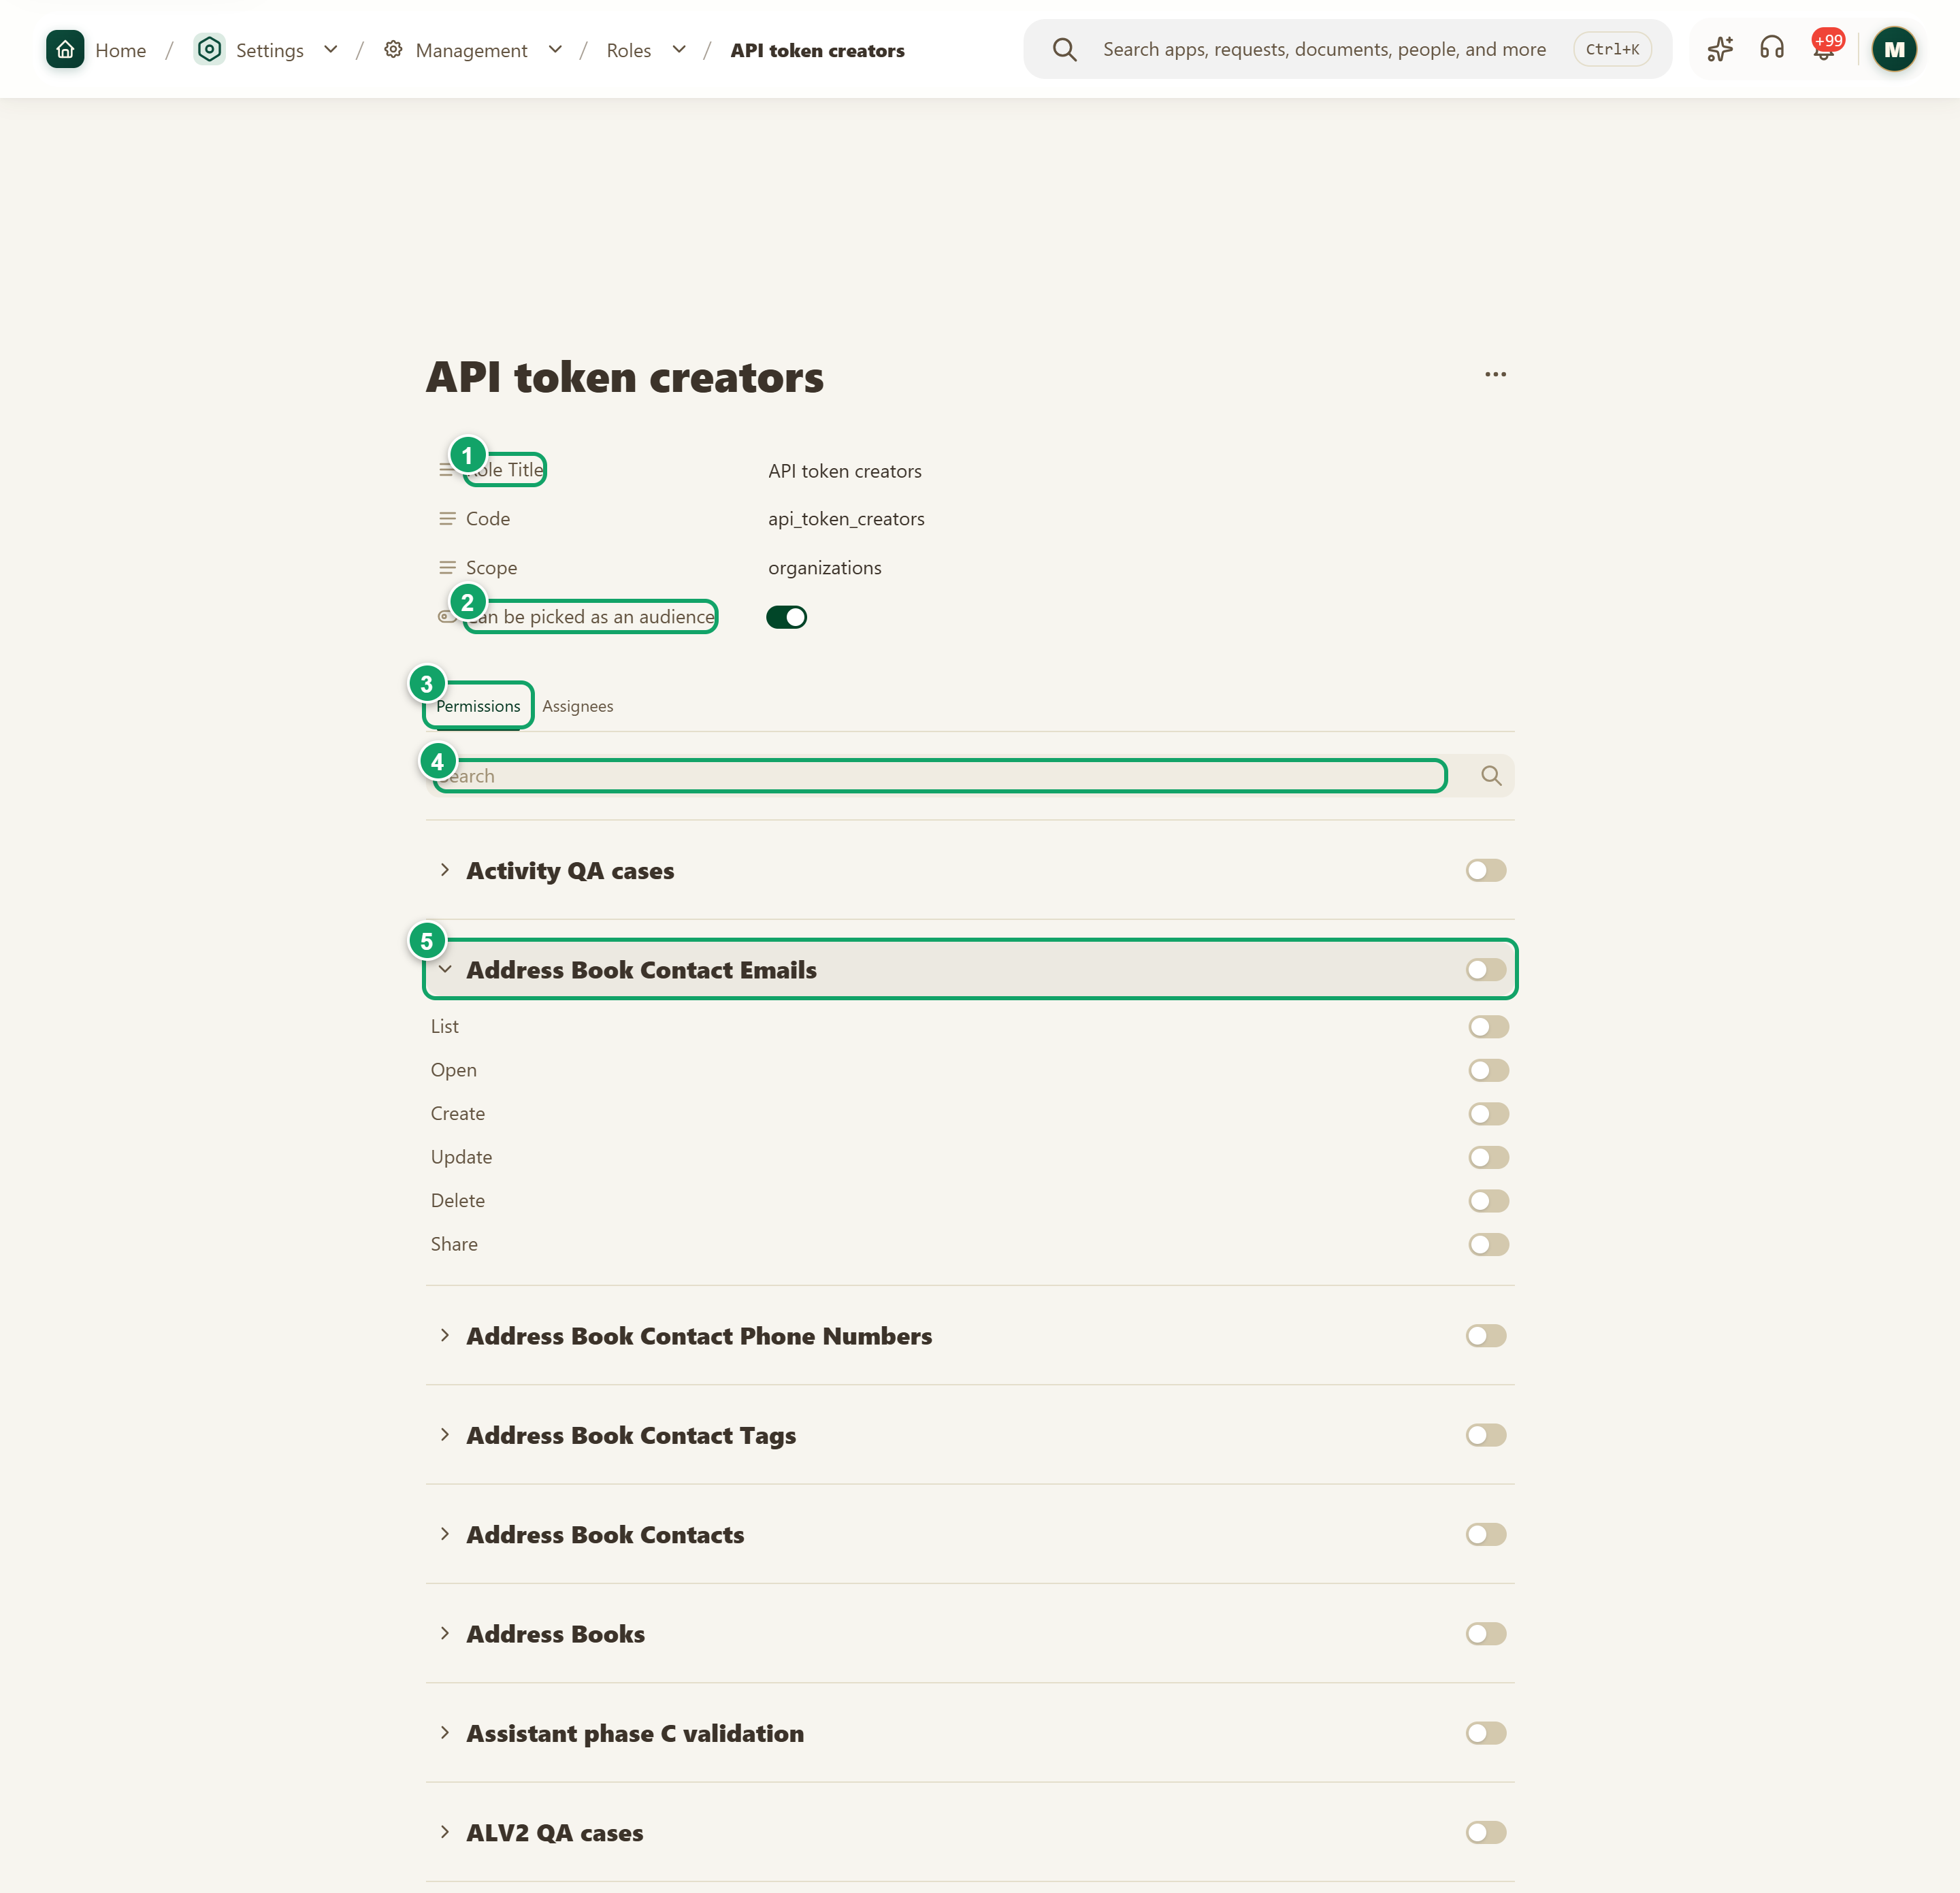
\includegraphics[width=0.95\linewidth,height=0.72\textheight,keepaspectratio]{figures/screens/ch08-roles-permissions-en.png}
\caption{The role page: “Permissions” tab}
\label{fig:settings-roles-permissions-screen}
\shotnote{This tab lists every record type the role can cover, and each row opens onto separate switches such as list, open, create and update. The role shown is a test role, opened to read only. ① “Role Title”. ② “Can be picked as an audience”: lets sharing and assignment pickers name the holders of this role, and saves as soon as you change it. ③ “Permissions”. ④ The search field: narrows the long list. ⑤ A record-type row: press its name to open it; the switch at its end turns all its permissions on together.}
\end{figure}

\begin{figure}[H]
\centering
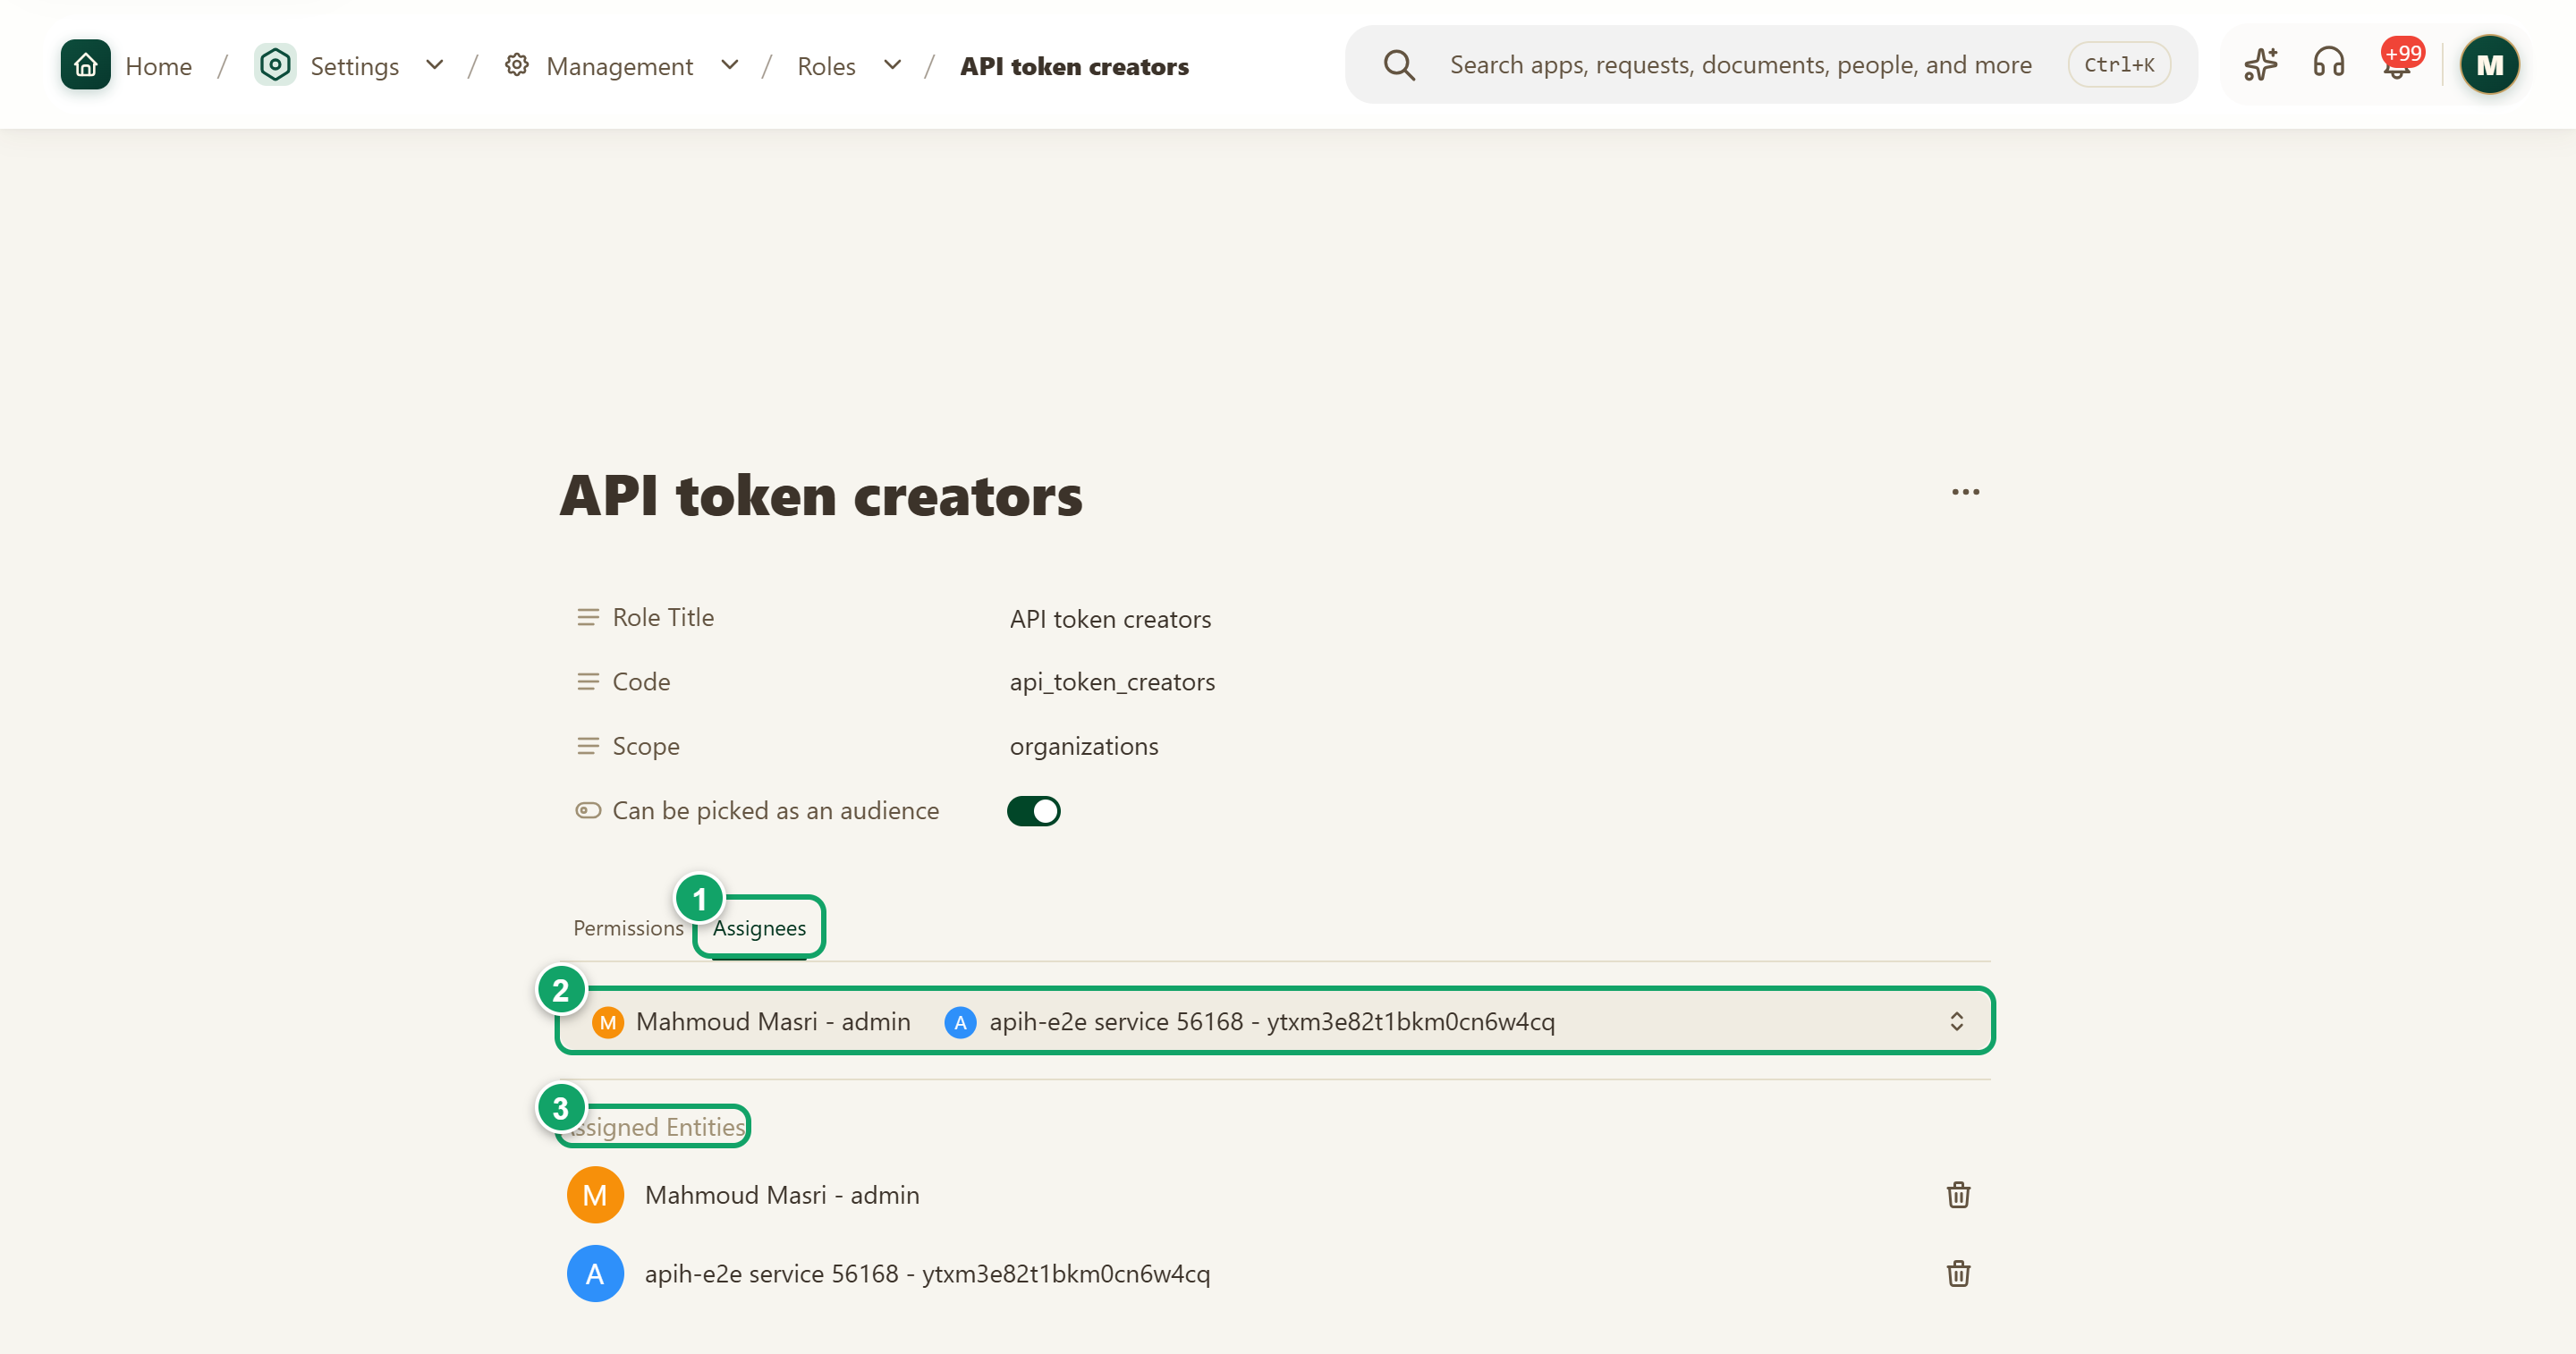
\includegraphics[width=0.95\linewidth,height=0.72\textheight,keepaspectratio]{figures/screens/ch08-roles-assignees-en.png}
\caption{The role page: “Assignees” tab}
\label{fig:settings-roles-assignees-screen}
\shotnote{A role does nothing until someone holds it, and this tab is where you assign it. Changes here are written straight away, while permission changes wait for “Save”. ① “Assignees”. ② The assignment field: choose a member, position or organizational unit. ③ “Assigned Entities”: who holds the role now; the delete button beside a name removes that assignment.}
\end{figure}

\begin{table}[H]
\centering
\caption{What do you record in a role?}
\label{tab:settings-roles-fields}
\begin{tabularx}{\linewidth}{R{4.2cm} Y}
\rcHeaderRow
\thh{Field} & \thh{What do you record?}\\
“Role Title” \req & A name that describes the responsibility. You can change it later.\\
“Code” \opt & The role’s identifier. Left empty, the system builds it from the title. It cannot change after creation.\\
“Scope” & “Organizations” for the whole organization, a record type that allows it, or a specific form. It cannot change after creation.\\
“Can be picked as an audience” & On for a new role. Turn it off if sharing and assignment pickers should not offer this role.\\
“Assign to Creator” & Shown on record-type and form roles. Gives whoever creates an item this role on that item automatically.\\
“Specifier” & Shown when the record type has a hierarchy. Sets whether the role applies to the item itself, or to what is above or below it.\\
“Permissions” & The switches allowed for each record type. On roles tied to a unit, location or position, a “Records” choice may appear to limit them to one value of a field.\\
“Assignees” & The members, positions and organizational units that hold the role.\\
\end{tabularx}
\end{table}

\begin{figure}[H]
\centering
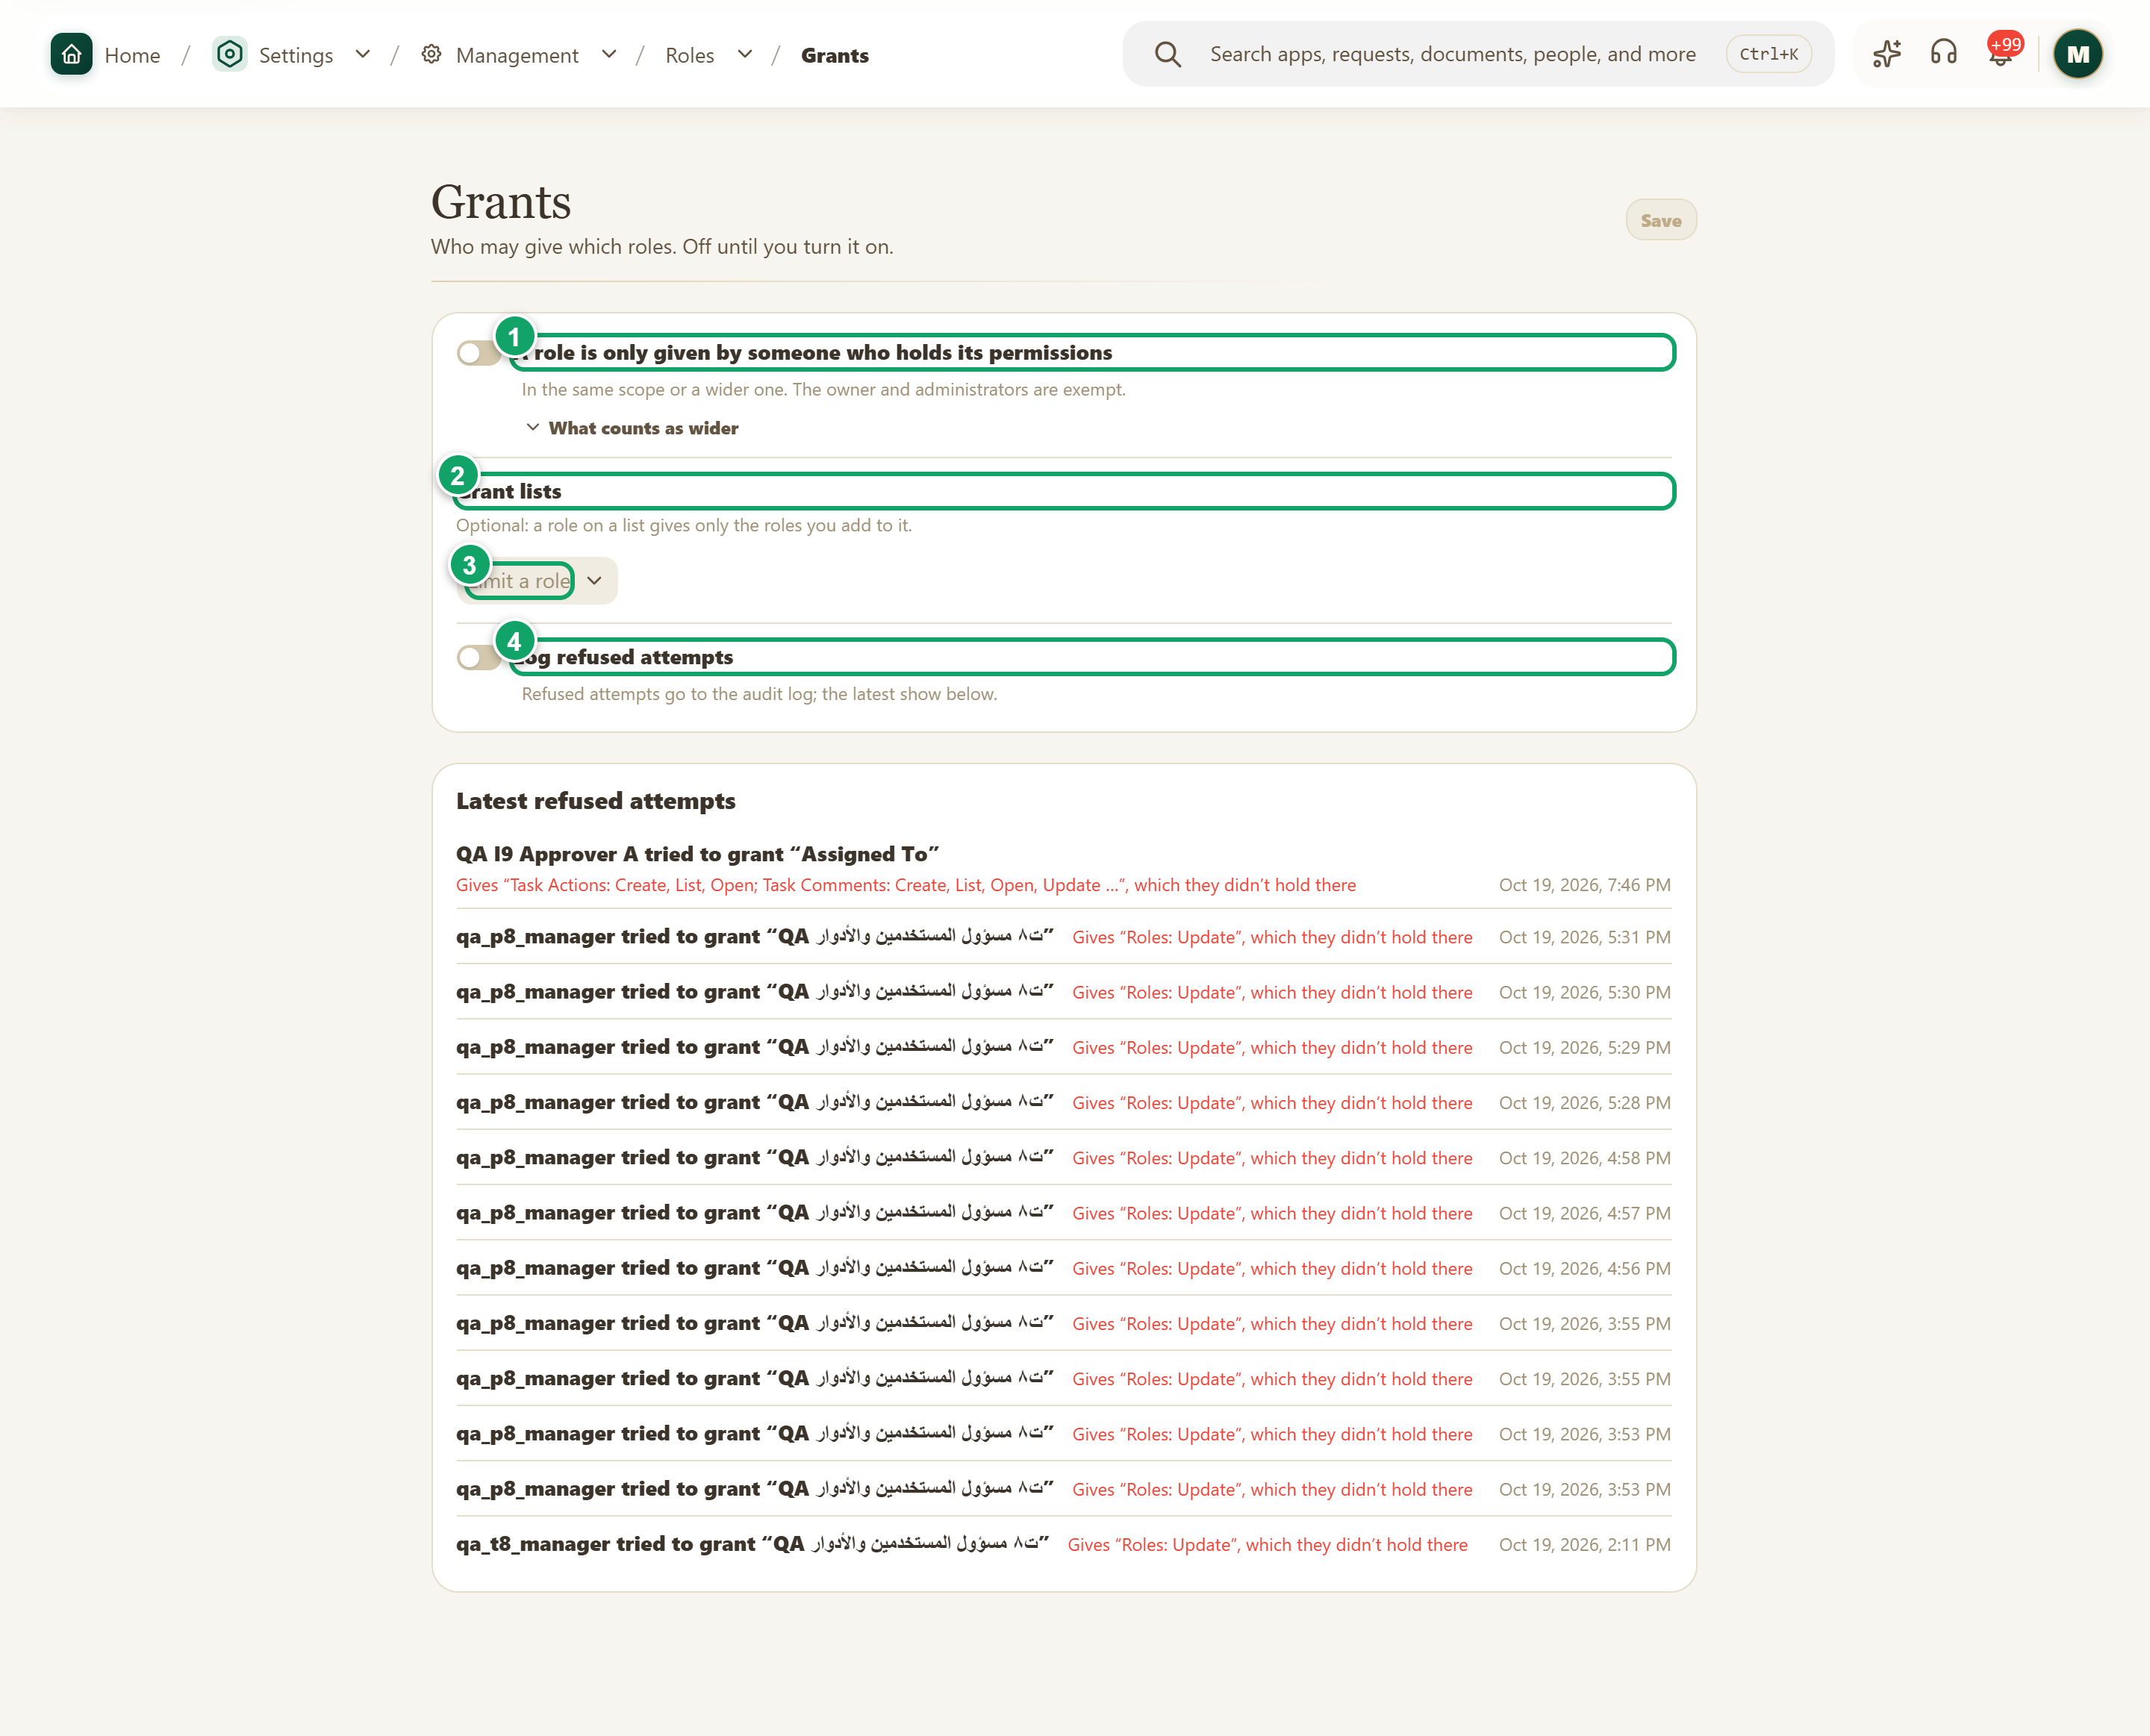
\includegraphics[width=0.95\linewidth,height=0.72\textheight,keepaspectratio]{figures/screens/ch08-roles-grants-en.png}
\caption{The “Grants” page}
\label{fig:settings-roles-grants-screen}
\shotnote{This page controls who may assign roles, not what the roles themselves allow. It stays off until you turn it on, and the lower list in the image shows refused test attempts. ① The main switch: stops anyone assigning a role with permissions they do not hold in the same or a wider scope; the owner and holders of the Administrator role are exempt. ② “Grant lists”. ③ “Limit a role”: restricts what a role’s holders can give to the roles you choose. ④ “Log refused attempts”.}
\end{figure}

\begin{enumerate}
\item Press “Add Role”, type the “Role Title”, choose the “Scope”, then press “Create Role”. The new role’s page opens.
\item In “Permissions”, search for the record type and press its name, then turn on only what is needed. The system also turns on what a permission depends on: turning on “Open” turns on “List” too.
\item Press “Save” in the “Unsaved changes” bar.
\item Open “Assignees” and add the members, positions or units.
\item To diagnose an access problem, open the three-dots menu beside “Grants” and choose “Debug user roles” or “Explain access”.
\item To delete a role, open it, press the three dots beside its title, choose “Delete Role” and confirm. Deleting cannot be undone, and a locked role cannot be deleted.
\end{enumerate}

\textbf{Check:} Reopen the role and confirm the switches stayed on and the right name appears in “Assigned Entities”. Then ask a member who holds the role to try the intended work and something that must stay denied; another role may give them the same permission.

\clearpage
\section{Two-step verification}
\label{sec:settings-feature-two-step}

Two-step verification adds a second proof after the password, so a stolen password is not enough to enter an account. The second step is either a code that changes every 30 seconds in an authenticator app on a phone, or a passkey saved on the member’s device, which counts as a second step on its own. This page is where you decide who needs it and follow who has finished setup. Only the organization’s owner and holders of the Administrator role can open it. Its settings affect how members sign in, so tell them before you change anything.

\begin{rcnote}[Example: Horizon]
Horizon’s system administrator chooses “Administrators” at ① and leaves a 14-day period at ②, protecting the widest accounts first. He then reviews the figure at ⑤ before extending the requirement to Sarah Al-Khatib and Omar Haddad.
\end{rcnote}

\begin{figure}[H]
\centering
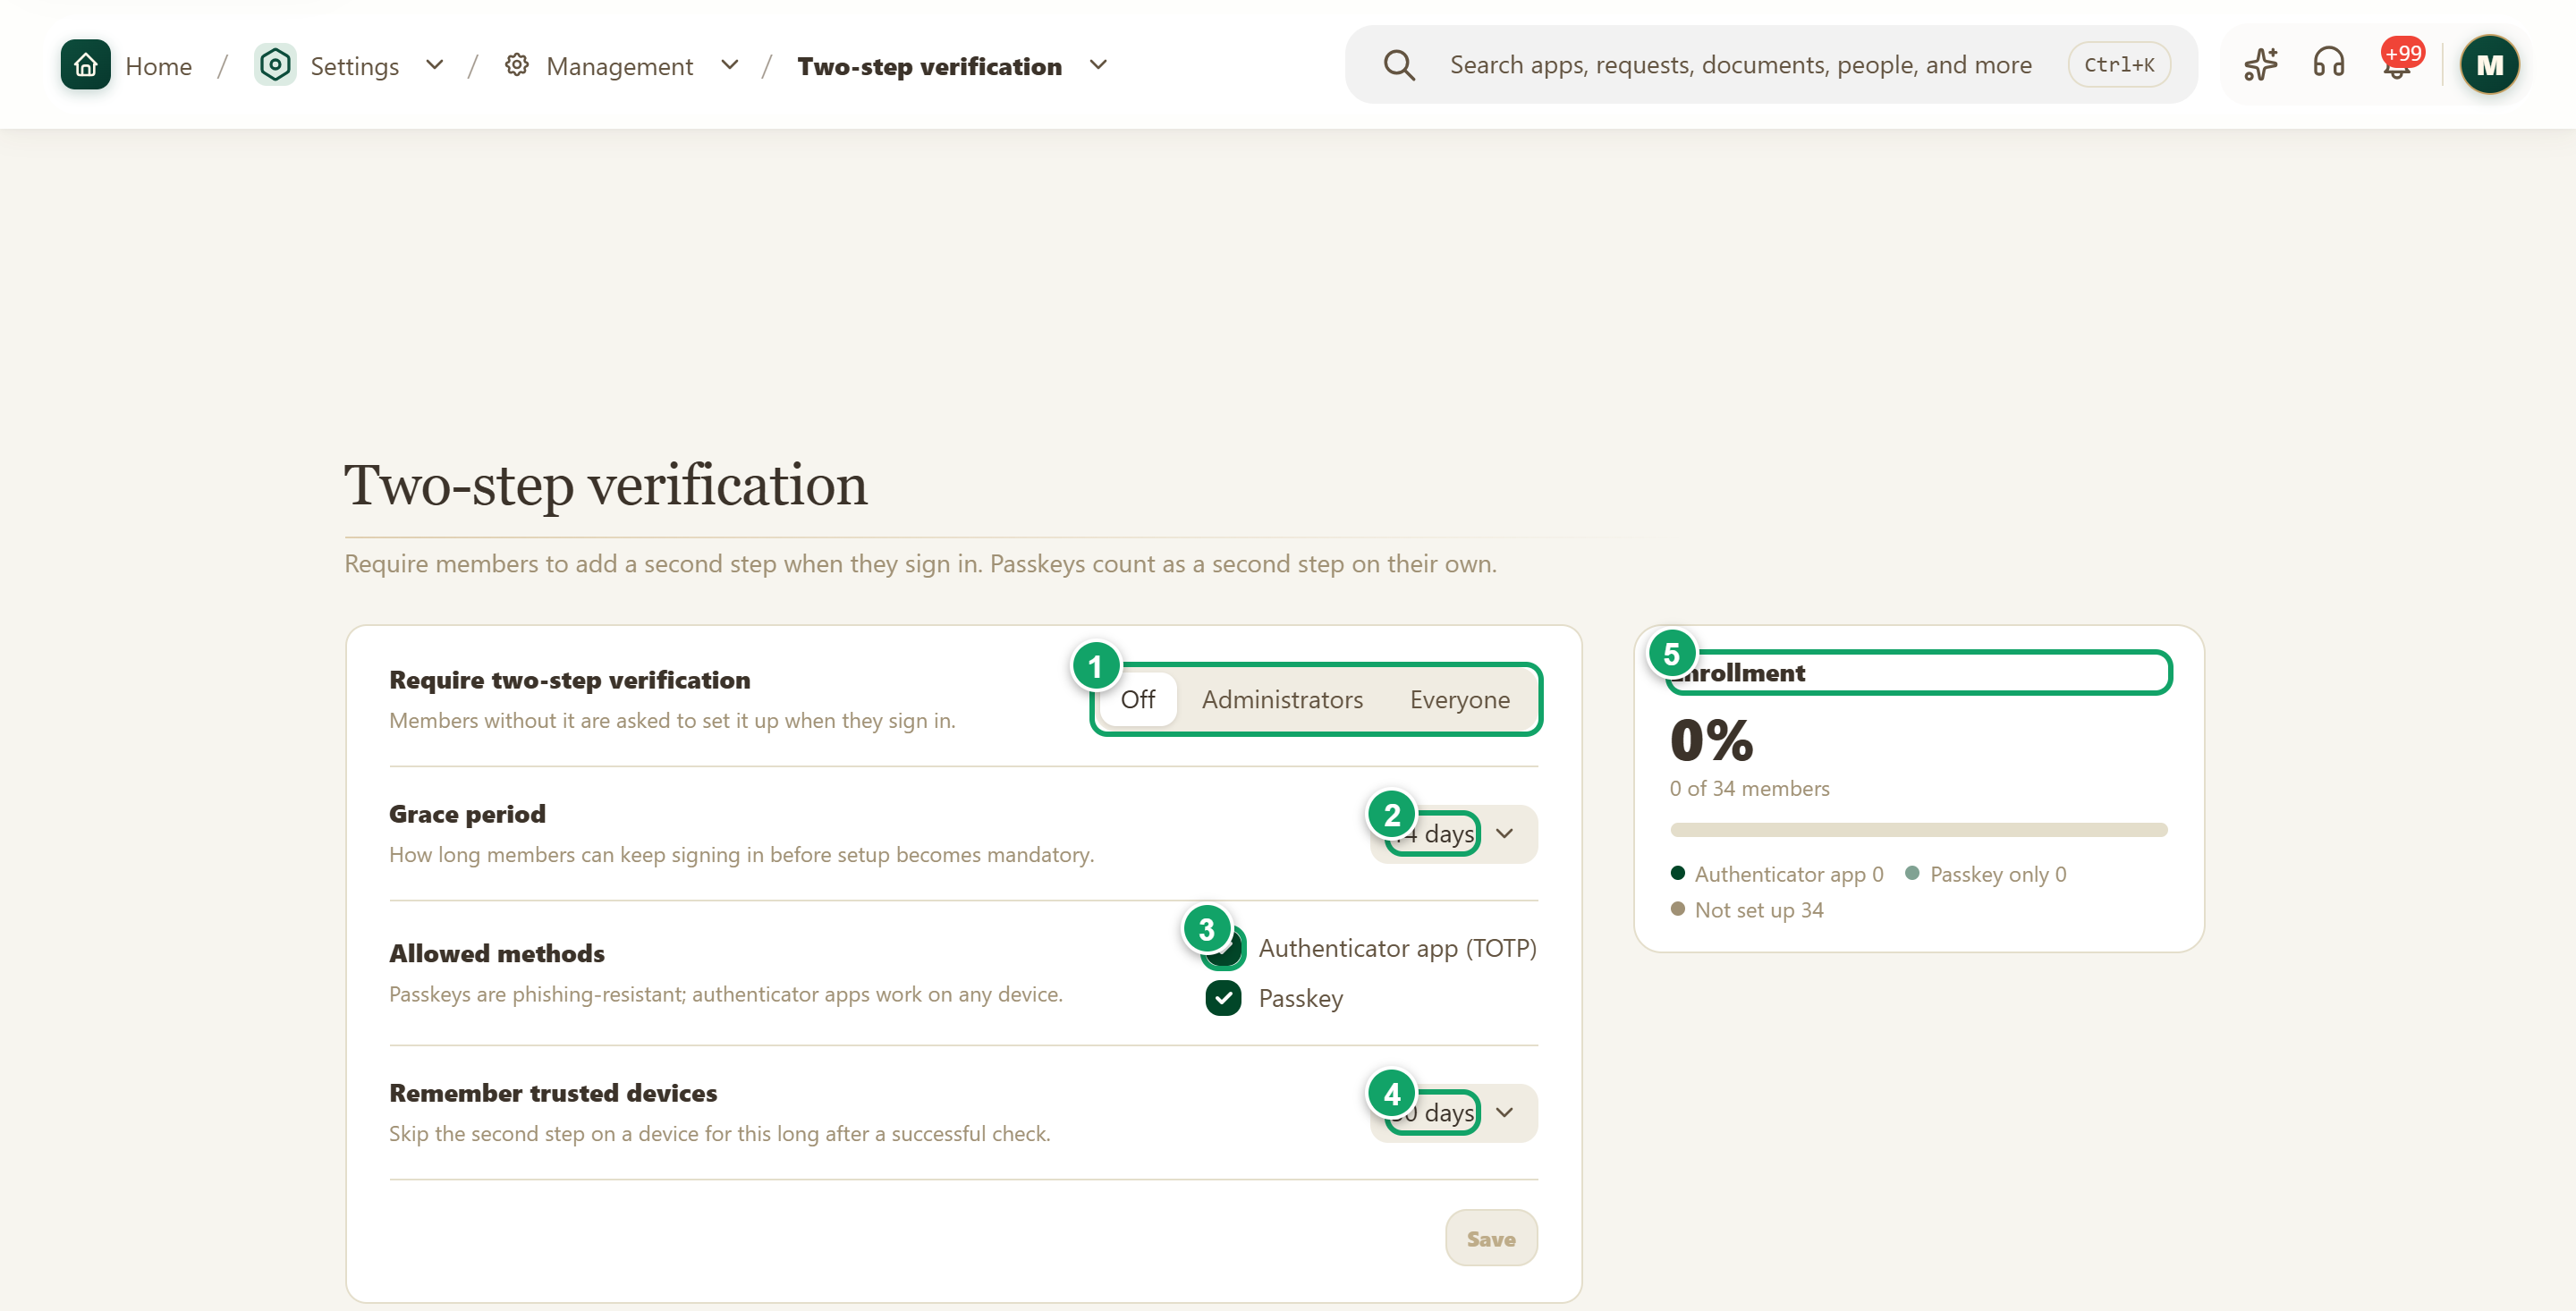
\includegraphics[width=0.95\linewidth,height=0.72\textheight,keepaspectratio]{figures/screens/ch08-two-step-en.png}
\caption{The two-step policy and enrollment figure}
\label{fig:settings-two-step-screen}
\shotnote{The page puts the organization’s decision beside its result: the settings in the large card, and how many members have the second step in the side card. The requirement is off in the test environment, so no list of pending members appears. ① “Require two-step verification”. ② “Grace period”. ③ “Allowed methods”: at least one must stay on. ④ “Remember trusted devices”. ⑤ “Enrollment”: a “Not set up yet” list appears under it once the requirement is on.}
\end{figure}

\begin{table}[H]
\centering
\caption{What do you record in the two-step policy?}
\label{tab:settings-two-step-fields}
\begin{tabularx}{\linewidth}{R{4.2cm} Y}
\rcHeaderRow
\thh{Field} & \thh{What do you record?}\\
“Require two-step verification” & “Off”, “Administrators” (the owner and holders of the Administrator role), or “Everyone”.\\
“Grace period” & “None”, or 7, 14 or 30 days. It counts from the day the requirement was turned on, or from the day a member was added if they joined later.\\
“Allowed methods” & “Authenticator app (TOTP)” and “Passkey”. You cannot turn both off.\\
“Remember trusted devices” & “Never”, or 7, 30 or 90 days: how long a device skips the second step after a successful check.\\
\end{tabularx}
\end{table}

\begin{enumerate}
\item Choose who the requirement covers, then the “Grace period”, “Allowed methods” and “Remember trusted devices”.
\item Press “Save”. Before saving, “Discard” returns the page to the last saved settings.
\item Follow the “Not set up yet” list, and press “Send reminder” beside a member or the group reminder button under the list.
\item If a member loses their phone, open their record and its “Two-step verification” tab, write the reason and press “Reset two-step verification”. This needs permission to reset the member’s password. It removes their authenticator app and recovery codes and signs them out; passkeys stay.
\end{enumerate}

\textbf{Check:} “Enrollment” rises as members finish setup, and those who have not show the days left. When the period ends, the member must set it up before finishing sign-in. If you turn off “Authenticator app (TOTP)”, however, setup is not forced at the end of the period on members without a passkey, so keep this method on if you want the requirement enforced.

\clearpage
\section{Sessions \& devices}
\label{sec:settings-feature-sessions}

A session is how long a member stays signed in on a device without typing the password again. A longer session is easier to work with; a shorter one lowers the risk from a forgotten or lost device. This page sets that balance for the whole organization: session length for each kind of device, sign-out after inactivity, the number of devices, and new-device alerts. Only the organization’s owner and holders of the Administrator role can open it. Changes apply to new sign-ins, not to sessions already open.

\begin{rcnote}[Example: Horizon]
Horizon’s system administrator lowers the web length at ① because some Aleppo Branch staff use shared computers, and keeps alerts on at ③. When Omar Haddad signs in on a new device, he is alerted. The administrator reviews the overall effect at ④ before saving.
\end{rcnote}

\begin{figure}[H]
\centering
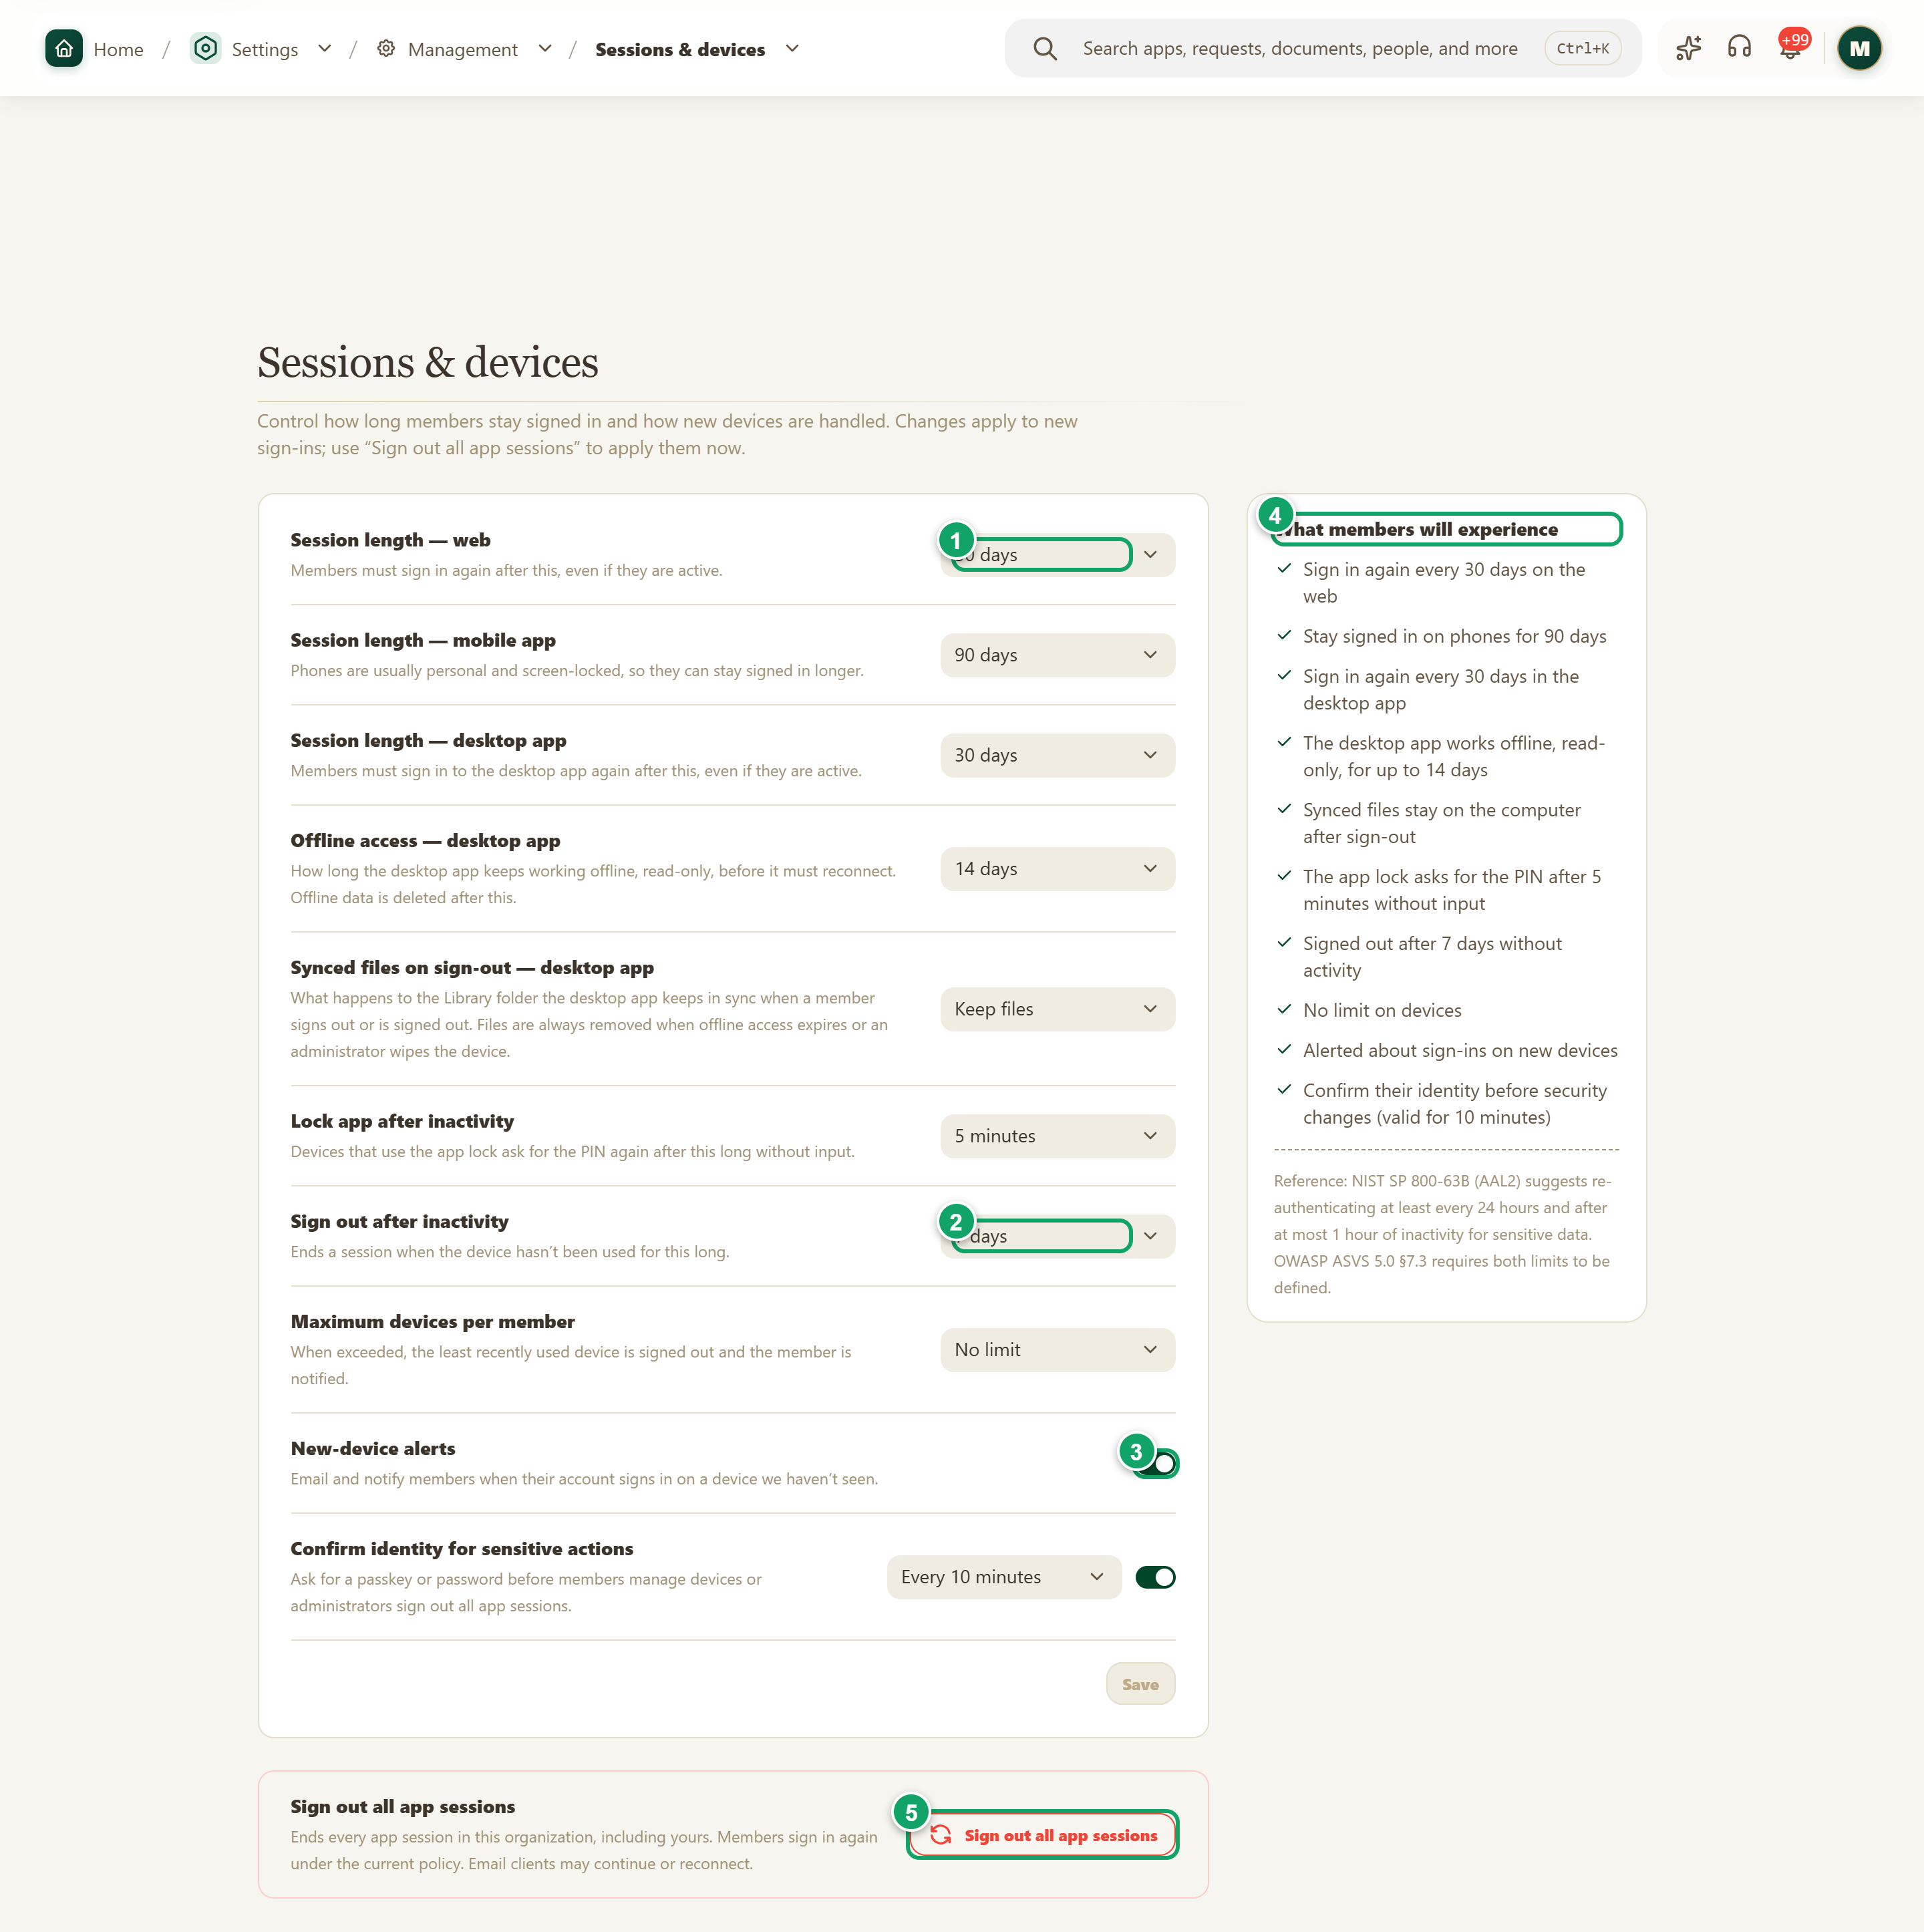
\includegraphics[width=0.95\linewidth,height=0.72\textheight,keepaspectratio]{figures/screens/ch08-sessions-en.png}
\caption{The sessions and devices policy}
\label{fig:settings-sessions-screen}
\shotnote{The side card turns the settings into what members will actually live with, and it changes with every choice before you save. The page shows the test environment’s current values, and nothing was changed. ① “Session length — web”. ② “Sign out after inactivity”. ③ “New-device alerts”. ④ “What members will experience”. ⑤ “Sign out all app sessions”: signs everyone out at once, including you.}
\end{figure}

\begin{table}[H]
\centering
\caption{What do you record in the session policy?}
\label{tab:settings-sessions-fields}
\begin{tabularx}{\linewidth}{R{4.2cm} Y}
\rcHeaderRow
\thh{Field} & \thh{What do you record?}\\
“Session length — web” & From 8 hours to 30 days. Members sign in again after this, even if active.\\
“Session length — mobile app” & From 7 to 180 days.\\
“Session length — desktop app” & From 8 hours to 90 days.\\
“Offline access — desktop app” & From 1 to 30 days of read-only work; offline data is then deleted if the device has not connected.\\
“Synced files on sign-out — desktop app” & Keep the Library folder’s files on the device, or remove them at sign-out.\\
“Lock app after inactivity” & From 1 minute to 1 hour, or “Never”. Applies to devices that use the app lock.\\
“Sign out after inactivity” & “Off”, or from 30 minutes to 7 days.\\
“Maximum devices per member” & “No limit”, or 1, 3, 5 or 10. When exceeded, the least recently used device is signed out and the member is told.\\
“New-device alerts” & Sends an email and a notification on a sign-in from an unknown device.\\
“Confirm identity for sensitive actions” & Asks for a passkey or password before managing devices or signing out all sessions. You choose how long the check lasts: 5, 10 or 30 minutes.\\
\end{tabularx}
\end{table}

\begin{enumerate}
\item Change the values you need, and watch their effect in “What members will experience”.
\item Press “Save”, or “Discard” to return to the last saved settings.
\item To apply the policy now, or on a suspected breach, press “Sign out all app sessions”, type the value the confirmation window asks for, then confirm with the same button. The system may ask you to confirm your identity first.
\end{enumerate}

\textbf{Check:} A success message appears, “Unsaved changes” disappears, and the side card matches your choices. After “Sign out all app sessions” you are signed out and the sign-in page appears. Email clients may continue or reconnect, because this action covers app sessions.

\clearpage
\section{Member Keys}
\label{sec:settings-feature-member-keys}

A member key is what a member signs with electronically: an encrypted file they keep, opened with a six-digit PIN only they know. It belongs to formal signing, in flows such as signing requests and correspondence, and has nothing to do with signing in. This page does not show the file or the PIN. It shows the active key’s public record, and it is where a key is revoked when someone leaves, loses the file, or a leak is suspected. You need permission to update members, and the page applies to the members that permission covers.

\begin{rcnote}[Example: Horizon]
Sarah Al-Khatib tells the system administrator that Omar Haddad has lost his laptop. The administrator selects Omar at ①, checks his active key, then revokes it so no new signature can be made with it.
\end{rcnote}

\begin{figure}[H]
\centering
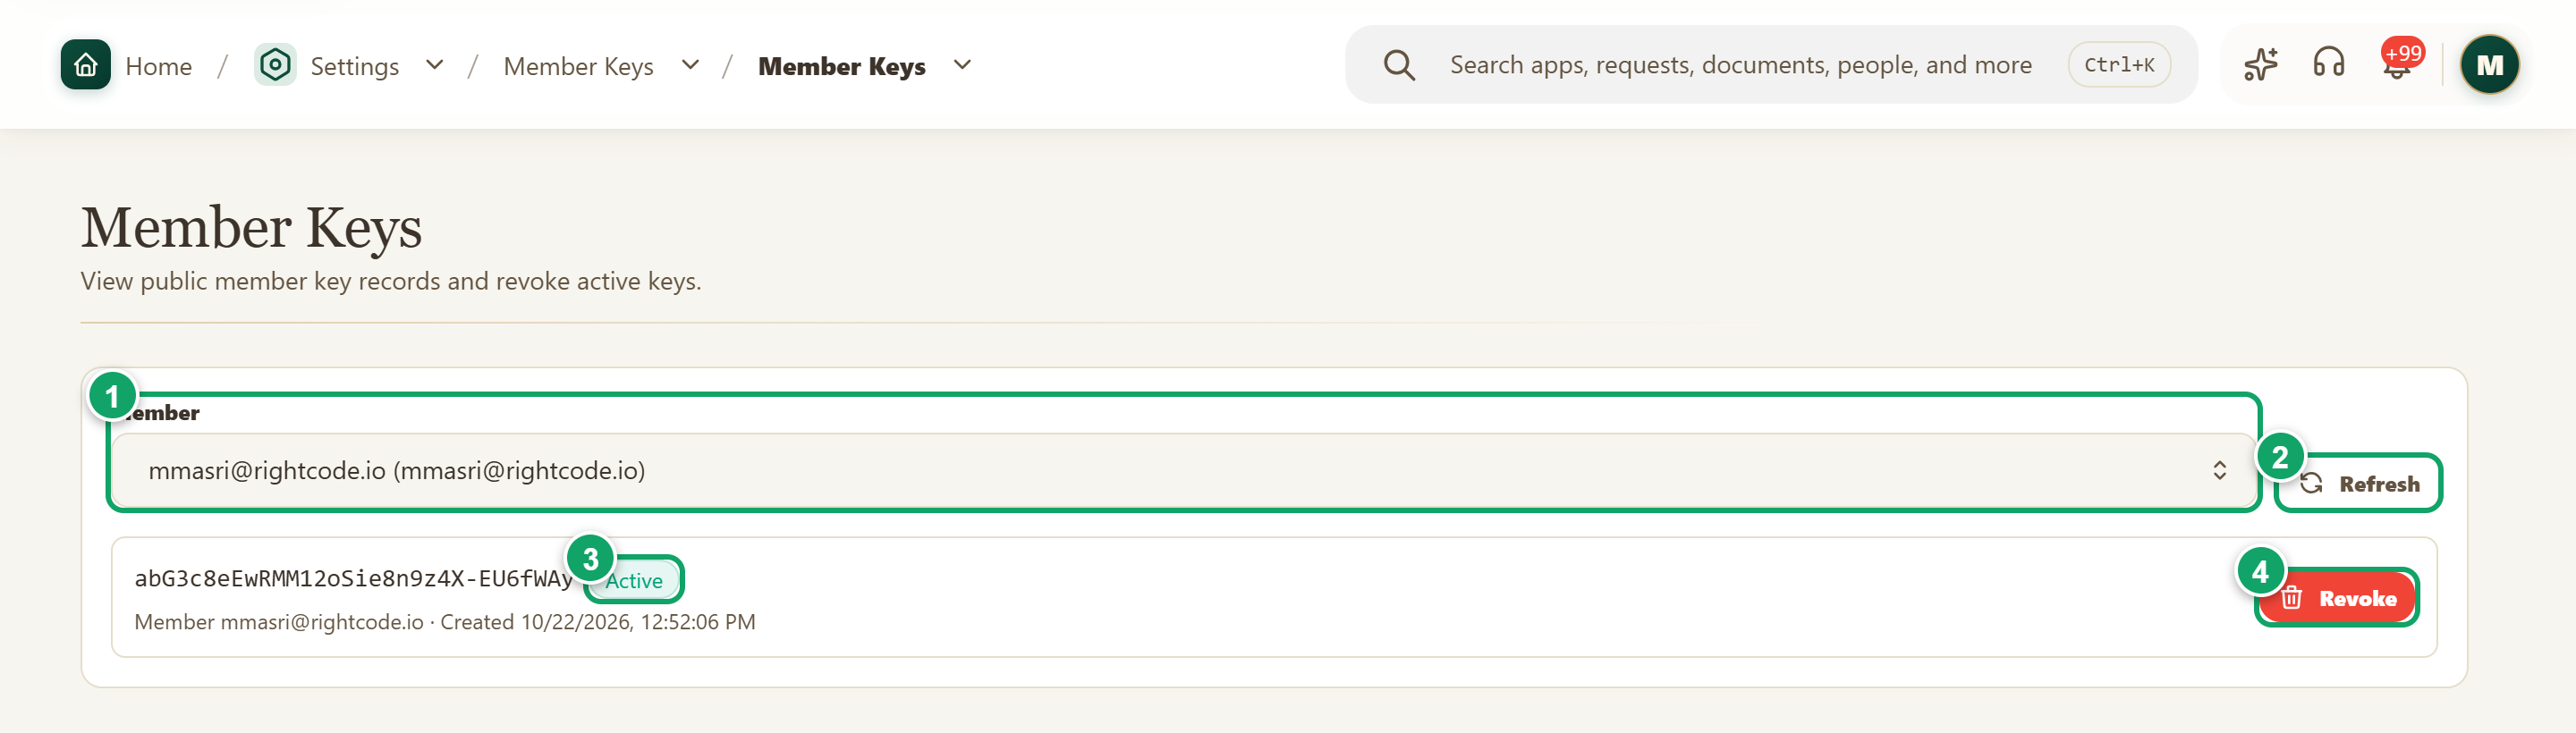
\includegraphics[width=0.95\linewidth,height=0.72\textheight,keepaspectratio]{figures/screens/ch08-member-keys-en.png}
\caption{A member’s keys on the “Member Keys” page}
\label{fig:settings-member-keys-screen}
\shotnote{The page starts empty with “No member keys registered.” until you choose a member, then shows only their active keys, with each key’s identifier and creation date. The identifier is a public label, not the key itself, and the key shown belongs to a test account. ① “Member”. ② “Refresh”. ③ The key’s status. ④ “Revoke”: stops the key and takes it off this list.}
\end{figure}

\begin{table}[H]
\centering
\caption{What does a key’s status mean?}
\label{tab:settings-member-keys-status}
\begin{tabularx}{\linewidth}{R{4.2cm} Y}
\rcHeaderRow
\thh{Status} & \thh{What does it mean?}\\
“Active” & The key can sign. This is the only status shown in “Member Keys”.\\
“Superseded” & The member registered a newer key, which replaced this one automatically. The member sees it in “Signature Management”.\\
“Revoked” & An administrator stopped it or the member disabled it. It cannot make a new signature. The member sees it in “Signature Management”.\\
\end{tabularx}
\end{table}

\begin{enumerate}
\item Choose the person in “Member”, and check the name and email; names can be alike.
\item Review the active key, and press “Refresh” if the member has just registered one.
\item To stop a key, press “Revoke” beside it, then confirm in the “Revoke Member Key” window.
\item If the member needs a new key, issue an enrollment token from the “Issue Enrollment Token” page (\ref{sec:settings-feature-key-enrollments}).
\end{enumerate}

\textbf{Check:} The key leaves the list, and “Audit Log” records “Credential Revoked”. Revoking does not change what was already signed and does not end pending signing requests, so redistribute those through their own flow.

\clearpage
\section{Issue Enrollment Token}
\label{sec:settings-feature-key-enrollments}

A member can create a signing key only with an enrollment token issued by an administrator. An enrollment token is a short-lived string of characters: it expires after 15 minutes, works once, and works only for the member it was issued to. The administrator can therefore confirm the member’s identity before enrollment, while the member generates the key alone without anyone seeing it. Use this page for a first enrollment or to replace a lost key. It needs permission to update members.

\begin{rcnote}[Example: Horizon]
The system administrator confirms Sarah Al-Khatib’s identity, selects her at ① and presses ②, then hands her the token directly. Sarah opens “Signature Management” straight away and finishes enrollment within the 15 minutes.
\end{rcnote}

\begin{figure}[H]
\centering
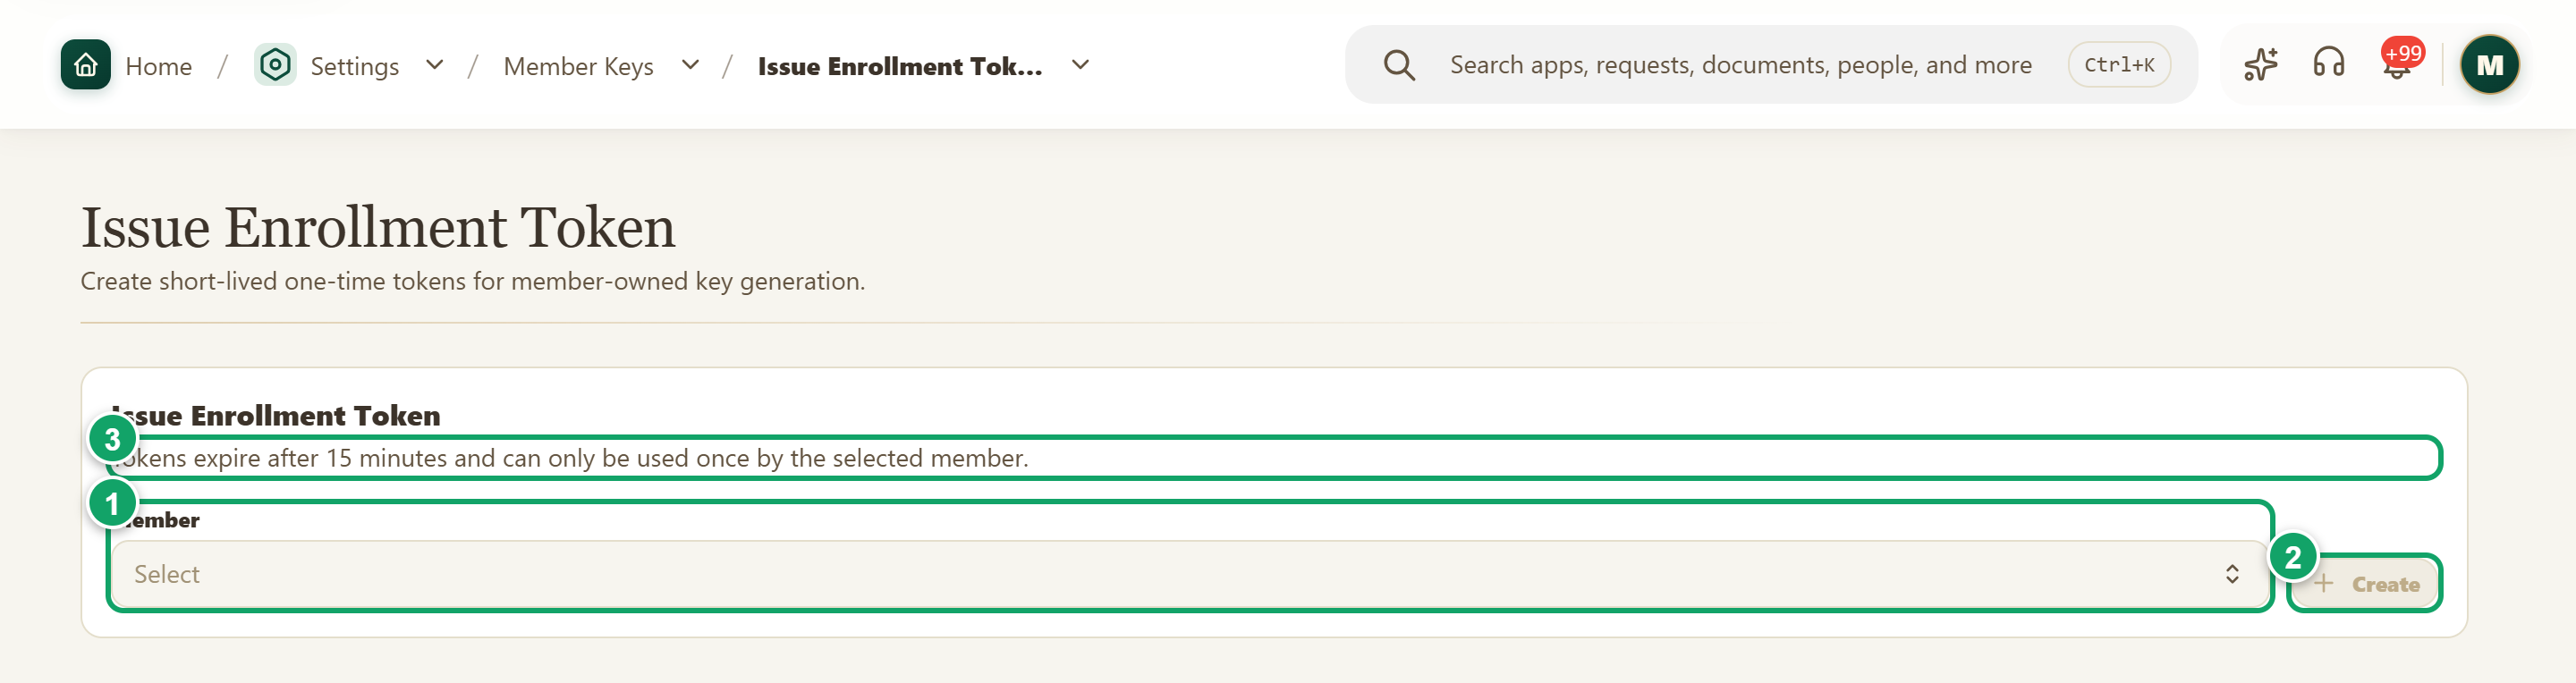
\includegraphics[width=0.95\linewidth,height=0.72\textheight,keepaspectratio]{figures/screens/ch08-key-enrollments-en.png}
\caption{Issuing an enrollment token to a member}
\label{fig:settings-key-enrollments-screen}
\shotnote{This short form ties the token to one member, and the create button stays disabled until one is chosen. No token was issued for this image, so it shows no real value. ① “Member”. ② “Create”: shows the token once, with a “Copy” button. ③ The validity rule: 15 minutes and one use.}
\end{figure}

\begin{figure}[H]
\centering
\begin{tikzpicture}[node distance=0.5cm]
\node[stepBox] (a) {Administrator confirms the member's identity};
\node[stepBox,below=of a] (b) {Administrator issues the token and hands it over safely};
\node[stepBox,below=of b] (c) {Member enters the token in Signature Management};
\node[stepBox,below=of c] (d) {Member chooses and confirms a PIN};
\node[stepBox,below=of d] (e) {Member draws a signature and downloads the file};
\node[stepBox,below=of e] (f) {Administrator confirms the key is Active};
\draw[flowsTo] (a) -- (b);
\draw[flowsTo] (b) -- (c);
\draw[flowsTo] (c) -- (d);
\draw[flowsTo] (d) -- (e);
\draw[flowsTo] (e) -- (f);
\end{tikzpicture}
\rclegend
\caption{The member key enrollment journey}
\label{fig:settings-key-journey-diagram}
\shotnote{The diagram shows where the work passes from administrator to member: the administrator starts the journey and checks its result, while the middle steps are done by the member alone. That is why the administrator never sees the PIN or the key file at any stage.}
\end{figure}

\begin{figure}[H]
\centering
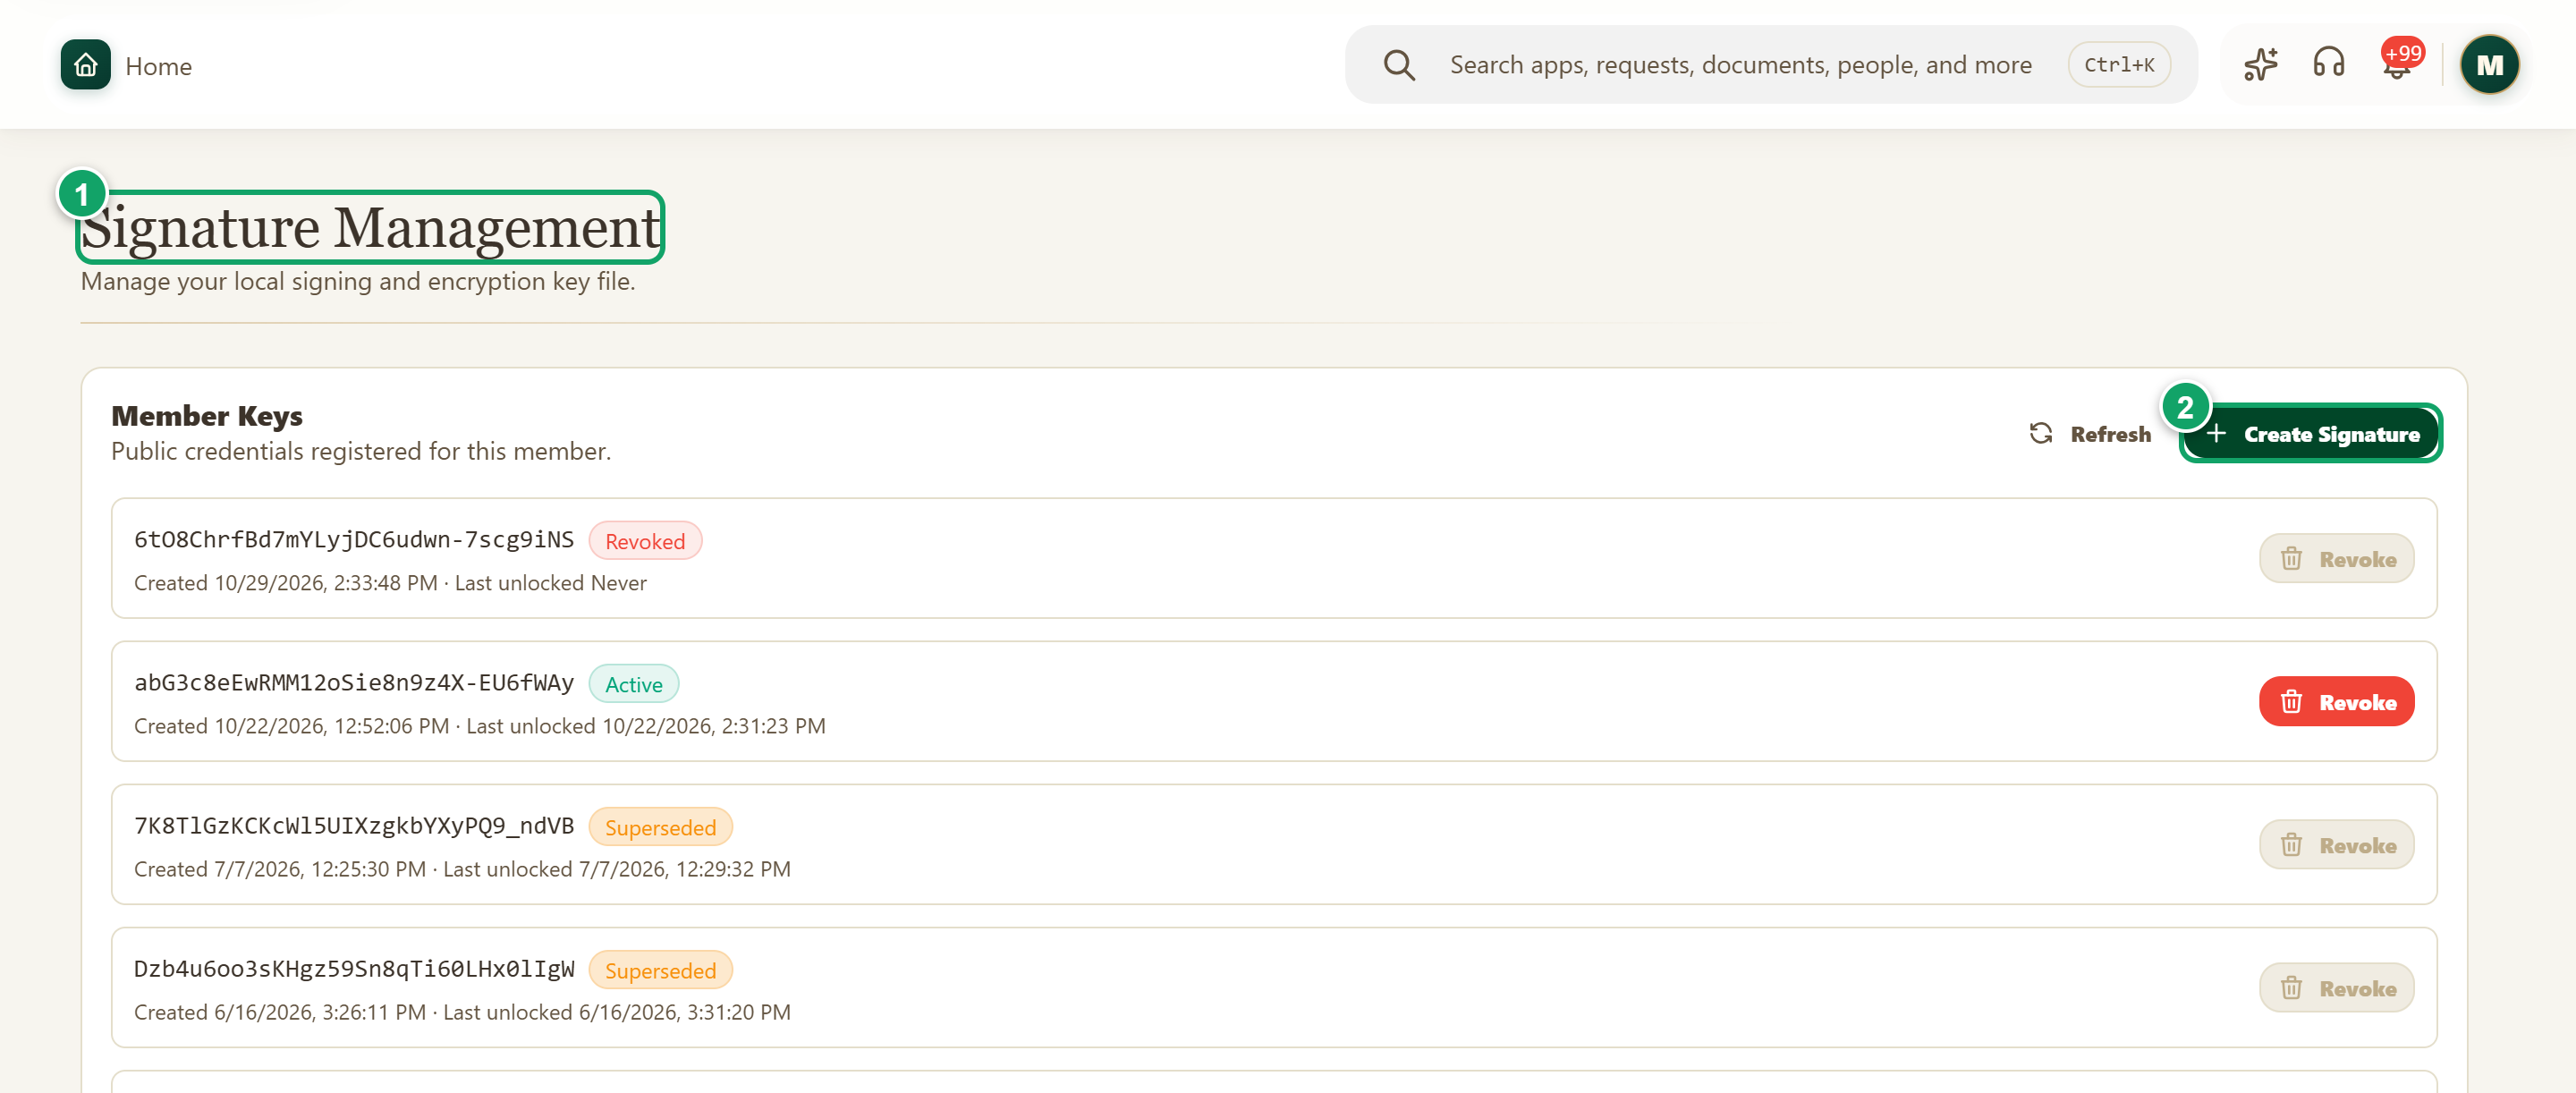
\includegraphics[width=0.95\linewidth,height=0.72\textheight,keepaspectratio]{figures/screens/ch08-key-member-en.png}
\caption{The “Signature Management” page, where the member finishes enrollment}
\label{fig:settings-key-member-screen}
\shotnote{This is the member’s personal page, not part of Settings. Here they use the token they received and see their keys in every status. They leave with a key file to keep somewhere private, because a lost file cannot be recovered. The keys shown belong to a test account. ① “Signature Management”. ② “Create Signature”: starts the four enrollment steps.}
\end{figure}

\begin{table}[H]
\centering
\caption{What does the member record in the “Create Signature” steps?}
\label{tab:settings-key-enrollments-fields}
\begin{tabularx}{\linewidth}{R{4.2cm} Y}
\rcHeaderRow
\thh{Step} & \thh{What do they record?}\\
“Enrollment Token” & The token the administrator handed over.\\
“PIN Setup” & Six digits, with no repeated digit, sequential digits or repeated pattern.\\
“Confirm PIN” & The same digits again.\\
“Draw Signature” & They draw their signature here, or press “Draw on Mobile” for a link valid for 5 minutes, then press “Create and Download”.\\
\end{tabularx}
\end{table}

\begin{enumerate}
\item Confirm the member’s identity, and prepare a safe way to hand over the token before issuing it.
\item Choose the member in “Member” and press “Create”.
\item Press “Copy” and hand the token to the member directly. Do not put it in a general chat, a ticket or a screenshot.
\item Ask the member to open “Signature Management”, press “Create Signature”, finish the steps and save the file.
\end{enumerate}

\textbf{Check:} A new key with “Active” status appears for the member in “Member Keys”, and “Audit Log” records “Enrollment Completed”. Any earlier active key becomes “Superseded”. If the token expires before the member finishes, issue a new token.

\clearpage
\section{Audit Log}
\label{sec:settings-feature-key-audit}

The audit log keeps what happened to one member’s keys: who issued the enrollment token, when the key was opened, whether attempts failed, and when it was revoked. Review it after a new enrollment, when you doubt a key’s use, or when a key is temporarily locked. It is read-only and needs permission to update members. It shows the latest 100 events for the chosen member.

\begin{rcnote}[Example: Horizon]
Omar Haddad reports that his key will not open. The system administrator selects him at ① and finds failed attempts followed by a temporary lockout, so he asks Omar to wait and check his PIN rather than issuing a new key.
\end{rcnote}

\begin{figure}[H]
\centering
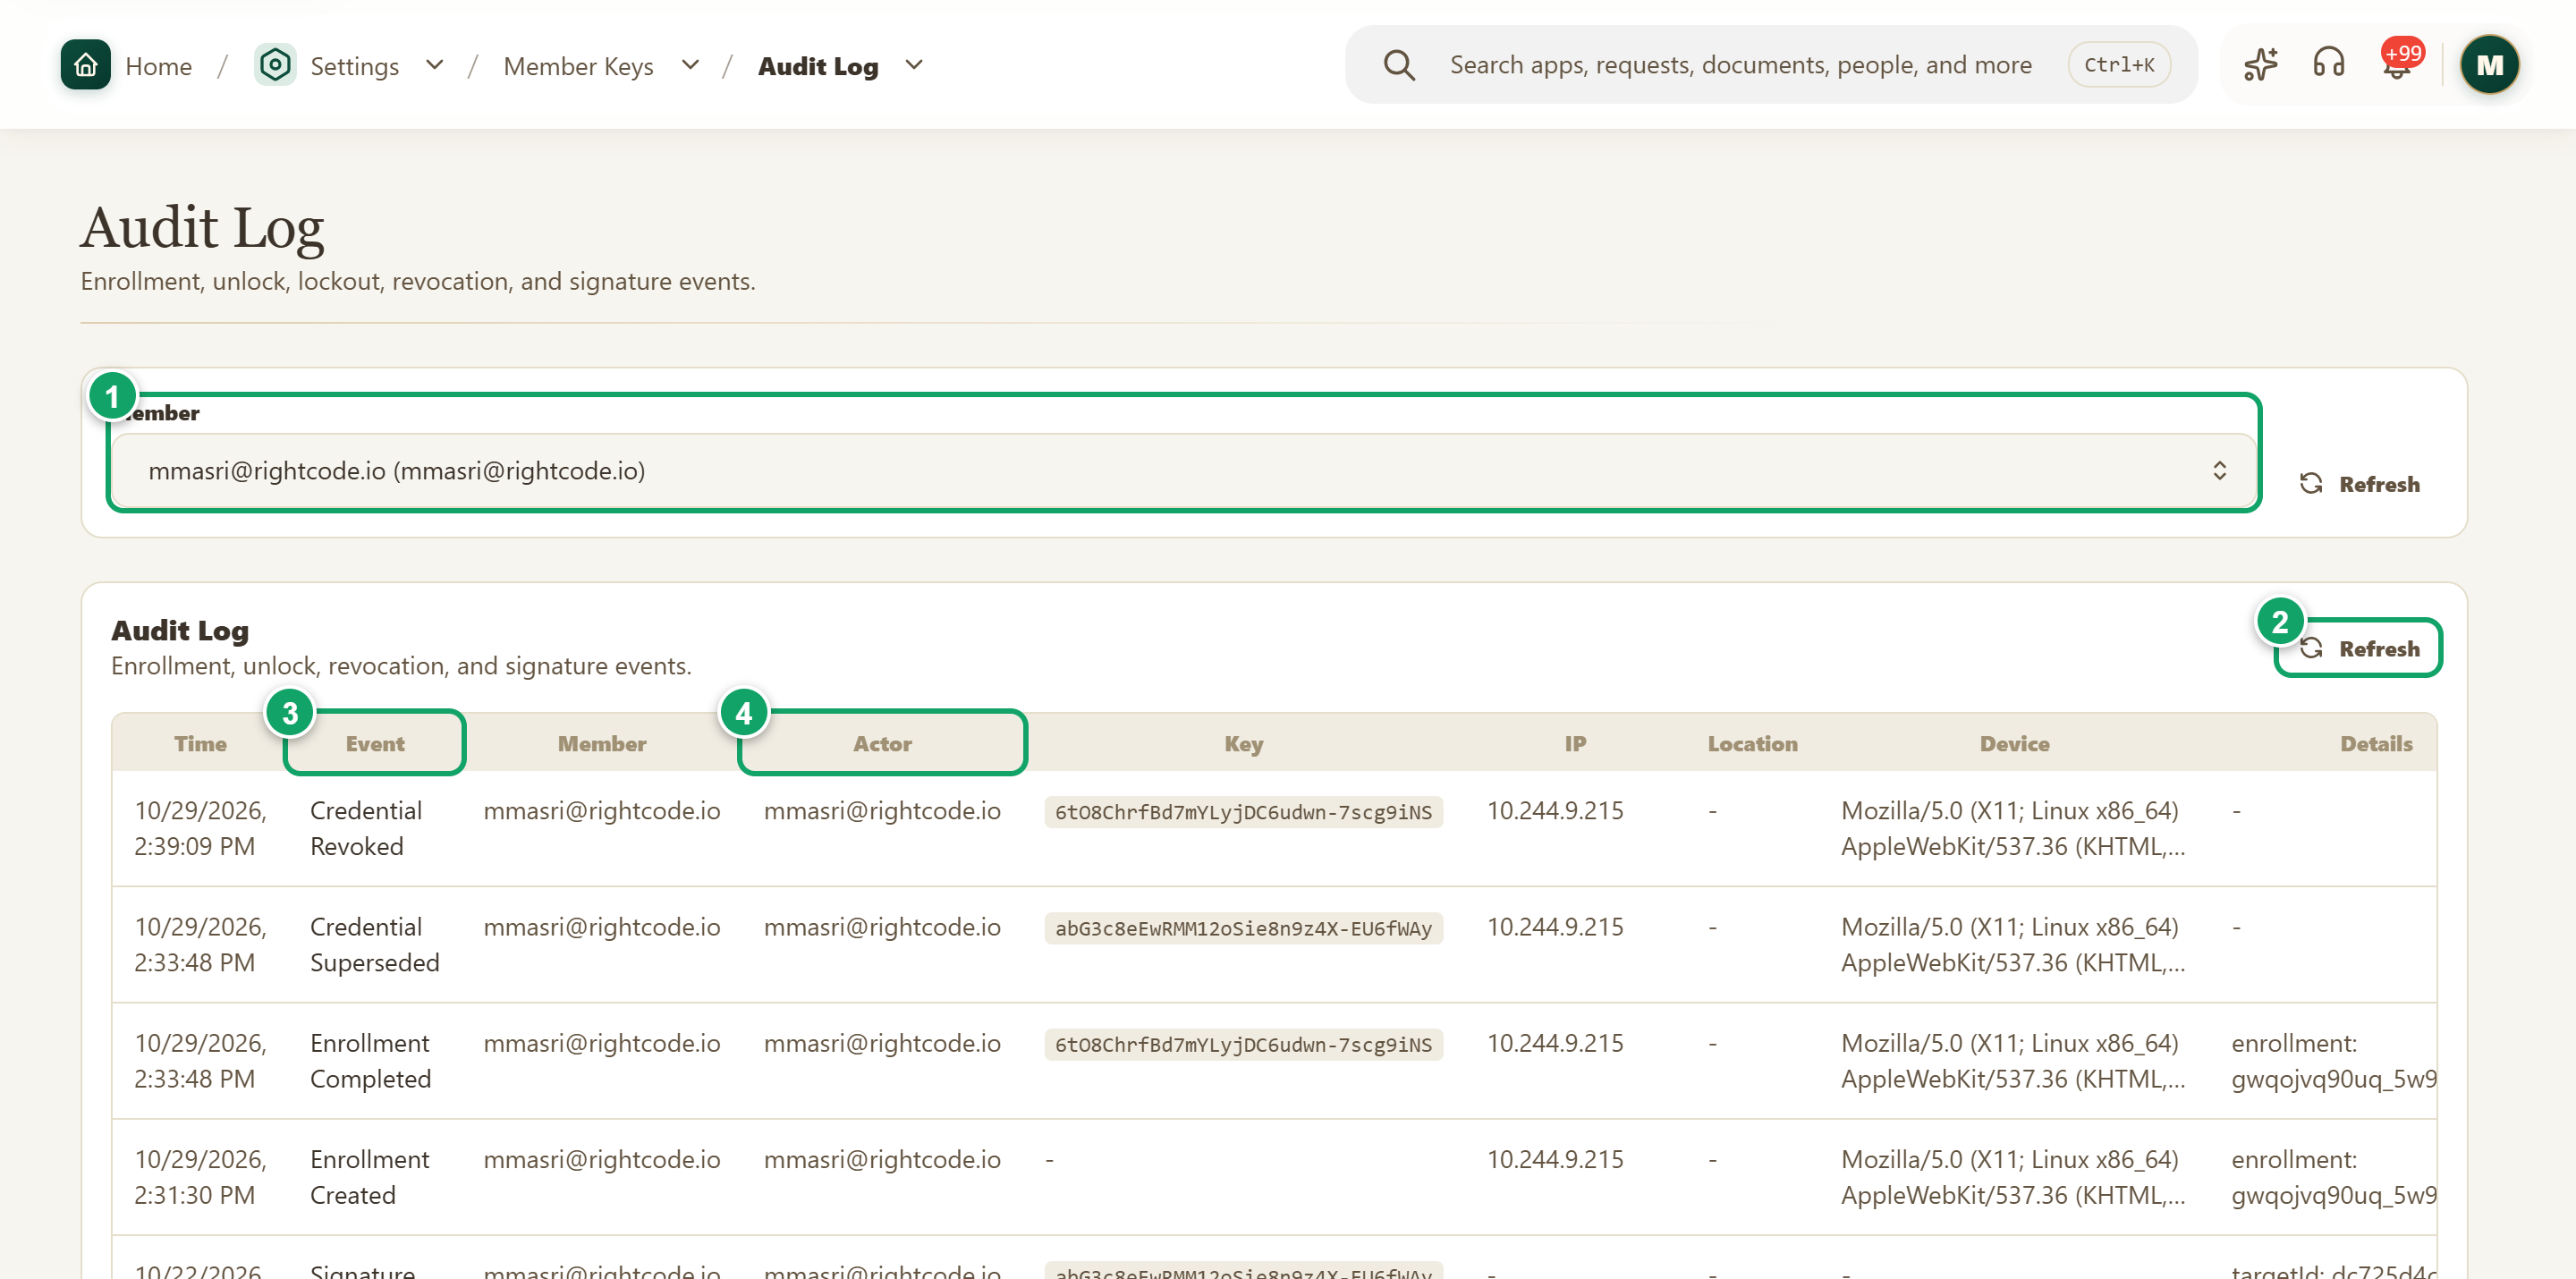
\includegraphics[width=0.95\linewidth,height=0.72\textheight,keepaspectratio]{figures/screens/ch08-key-audit-en.png}
\caption{The member key audit log}
\label{fig:settings-key-audit-screen}
\shotnote{The log stays empty until you choose a member, then shows a table, newest first, of each event’s time, type, actor, key and device. The events shown belong to a test account. ① “Member”. ② “Refresh”. ③ “Event”. ④ “Actor”: who performed the action, who may differ from the key’s owner.}
\end{figure}

\begin{table}[H]
\centering
\caption{What do the main log events mean?}
\label{tab:settings-key-audit-events}
\begin{tabularx}{\linewidth}{R{4.2cm} Y}
\rcHeaderRow
\thh{Event} & \thh{What does it mean?}\\
“Enrollment Created” and “Enrollment Completed” & A token was issued, then the member finished creating a key with it.\\
“Credential Superseded” and “Credential Revoked” & A new key replaced the old one, or someone stopped the key.\\
“Unlock Started”, “Unlock Succeeded” and “Unlock Failed” & An attempt to use the key with its file and PIN, and the result.\\
“Unlock Locked” & After five failed attempts the key locks for 30 minutes. This event also appears in English in the Arabic interface.\\
“Signature Handoff Submitted” & The signature drawing arrived from the phone through the temporary link.\\
\end{tabularx}
\end{table}

\begin{enumerate}
\item Choose the member in “Member”.
\item Read the events from the newest, and look at “Actor”, “IP”, “Location” and “Device”.
\item Press “Refresh” to fetch anything new.
\end{enumerate}

\textbf{Check:} The event you are looking for appears with its time and actor. If you see attempts the member does not recognize, revoke the key in “Member Keys” and issue a new token after confirming their identity.

\clearpage
\section{API \& integrations}
\label{sec:settings-feature-api}

The API is a door through which other systems reach the organization’s data without a person involved, such as a finance system reading records every night. The outside system enters with an API token: a long secret that decides who the system acts as and what it may do. This page gathers tokens, their owners, their activity and the general rules for them. Every member sees the “Tokens” tab and their own tokens; creating tokens and the other tabs depend on role permissions such as “Create API tokens” and “Manage API policy”.

\begin{rcnote}[Example: Horizon]
Horizon’s finance team asks to connect its system to KayanOS. The system administrator does not use Omar Haddad’s personal token. He presses “New service account” in the “Service accounts” tab, then creates a read-only token for the account, so the integration keeps working if any employee leaves.
\end{rcnote}

\begin{figure}[H]
\centering
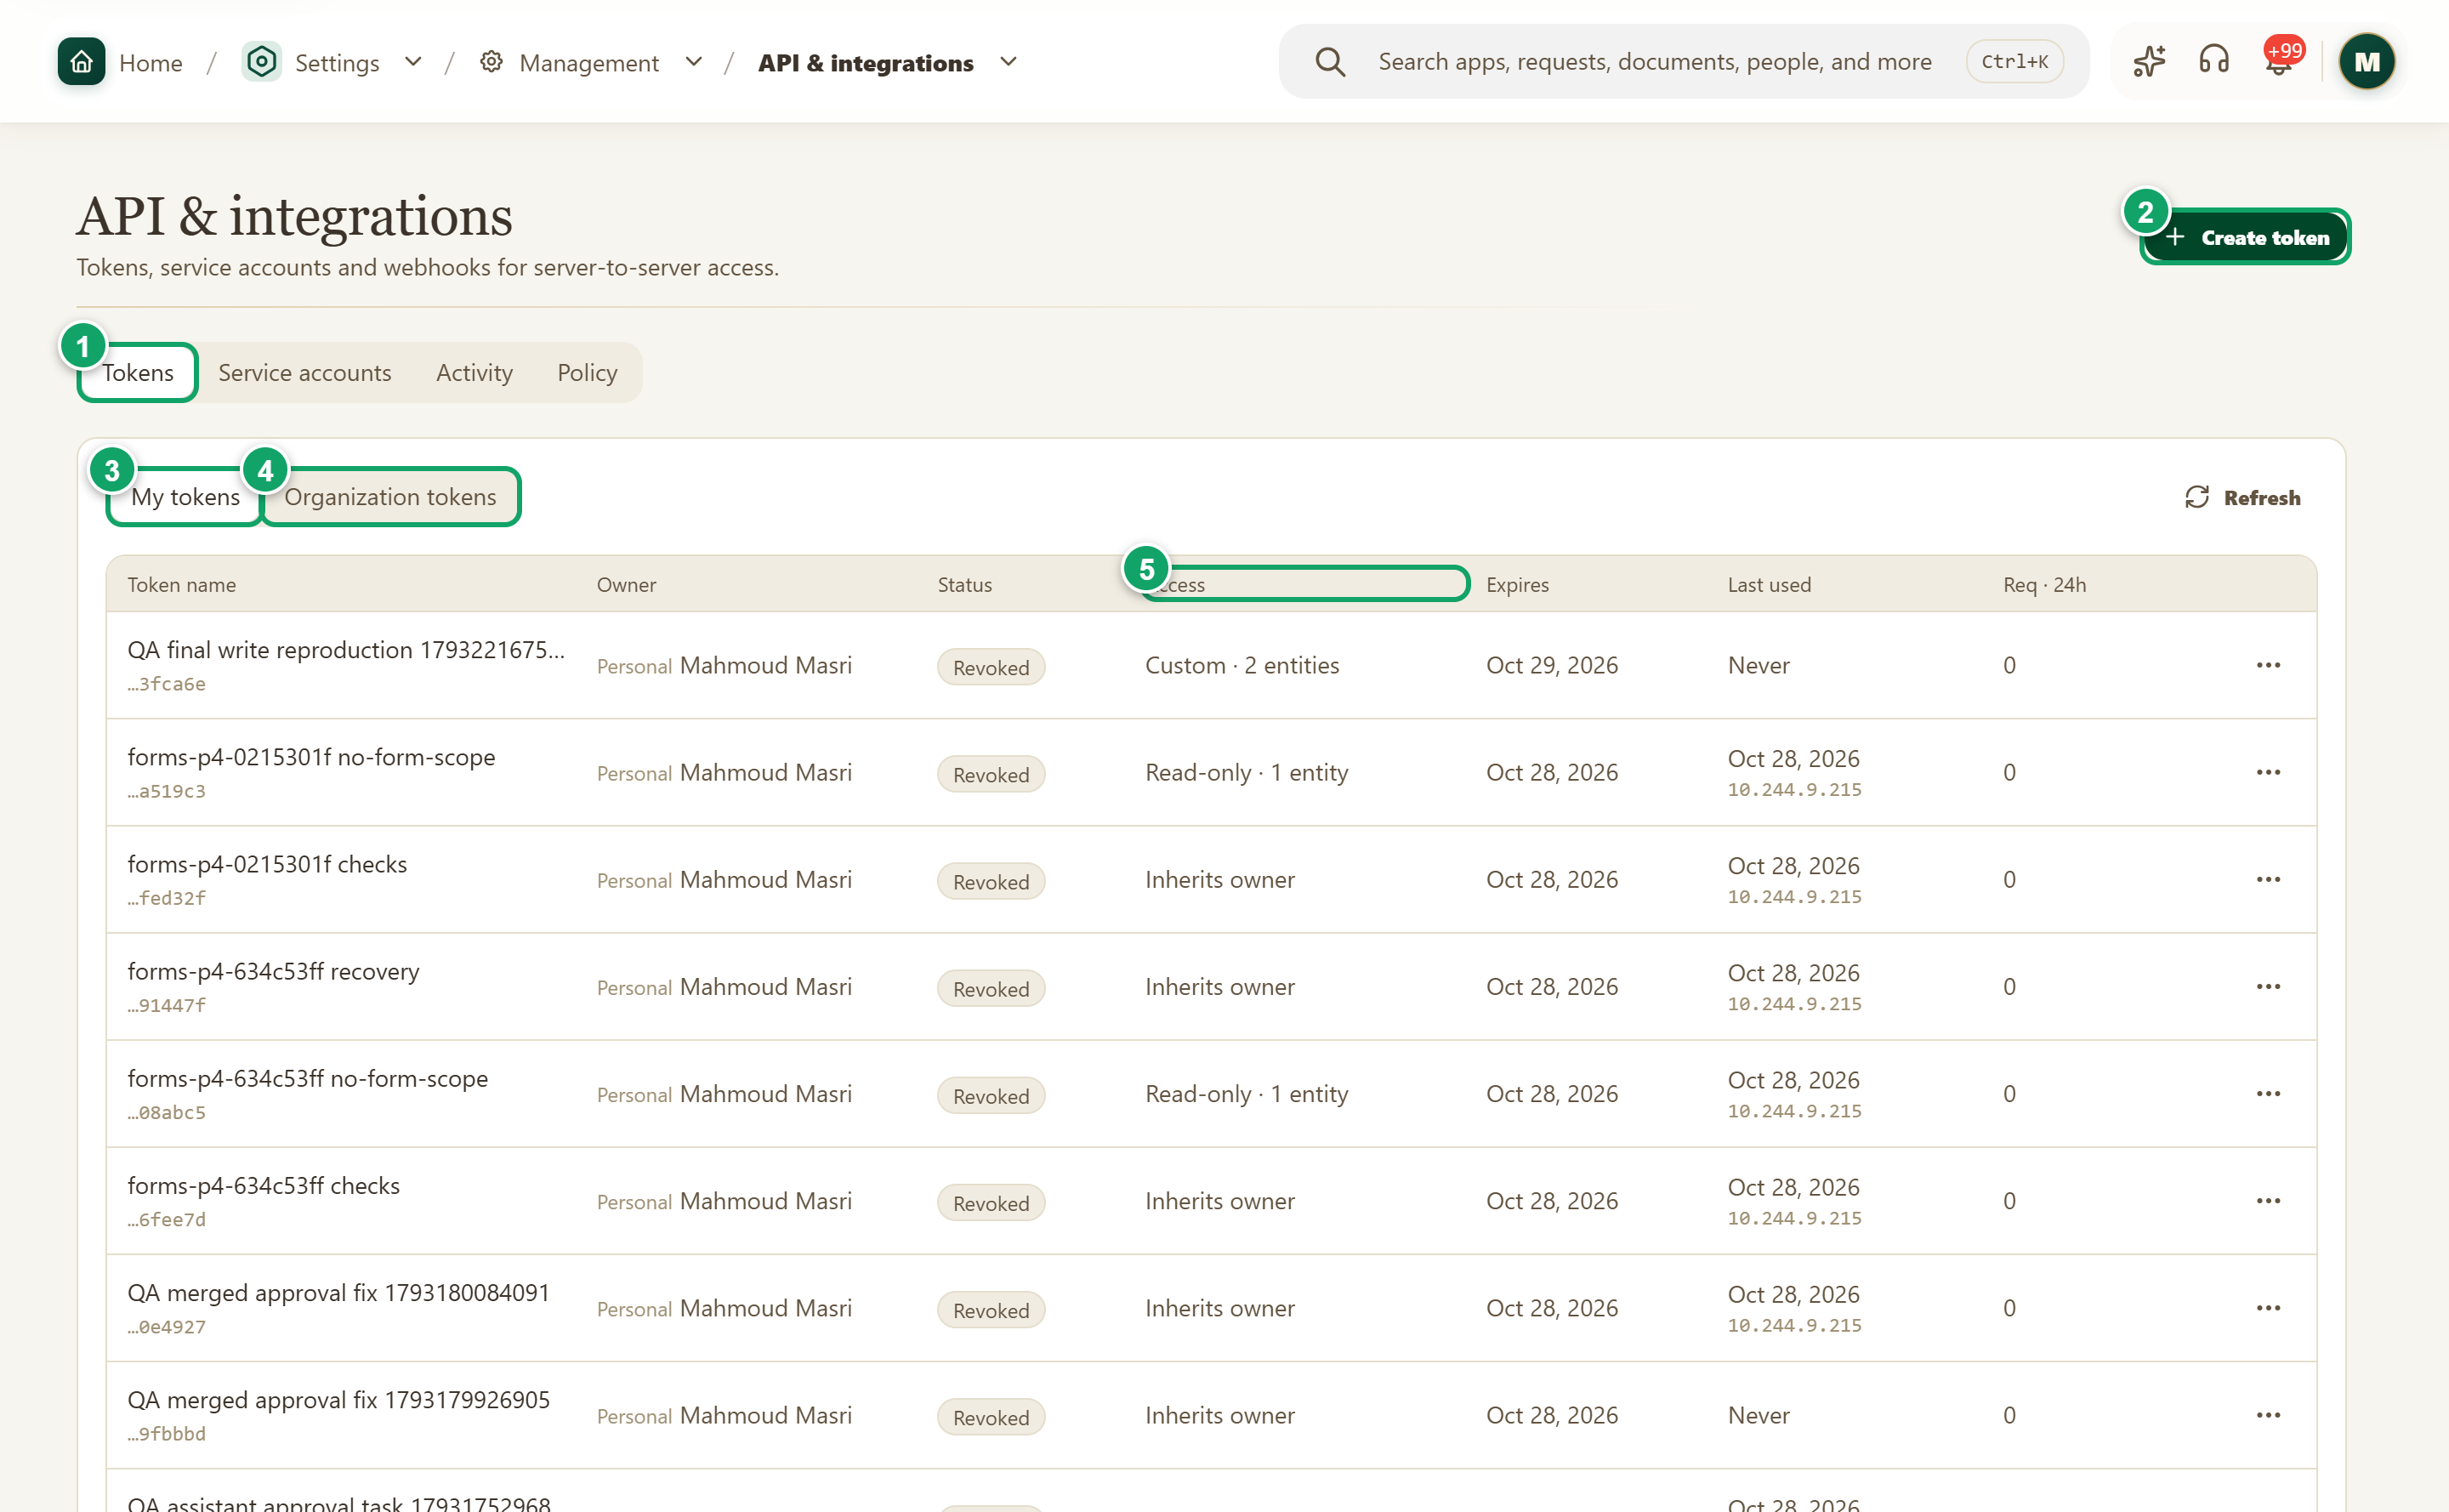
\includegraphics[width=0.95\linewidth,height=0.72\textheight,keepaspectratio]{figures/screens/ch08-api-tokens-en.png}
\caption{The “Tokens” tab}
\label{fig:settings-api-tokens-screen}
\shotnote{The table shows each token with its owner, status, access, expiry and last use. The token itself never appears, only a short ending; the tokens shown are revoked test tokens. ① “Tokens”. ② “Create token”. ③ “My tokens”. ④ “Organization tokens”: shown to those allowed to see them. ⑤ “Access”: a short summary of what the token can do.}
\end{figure}

\begin{figure}[H]
\centering
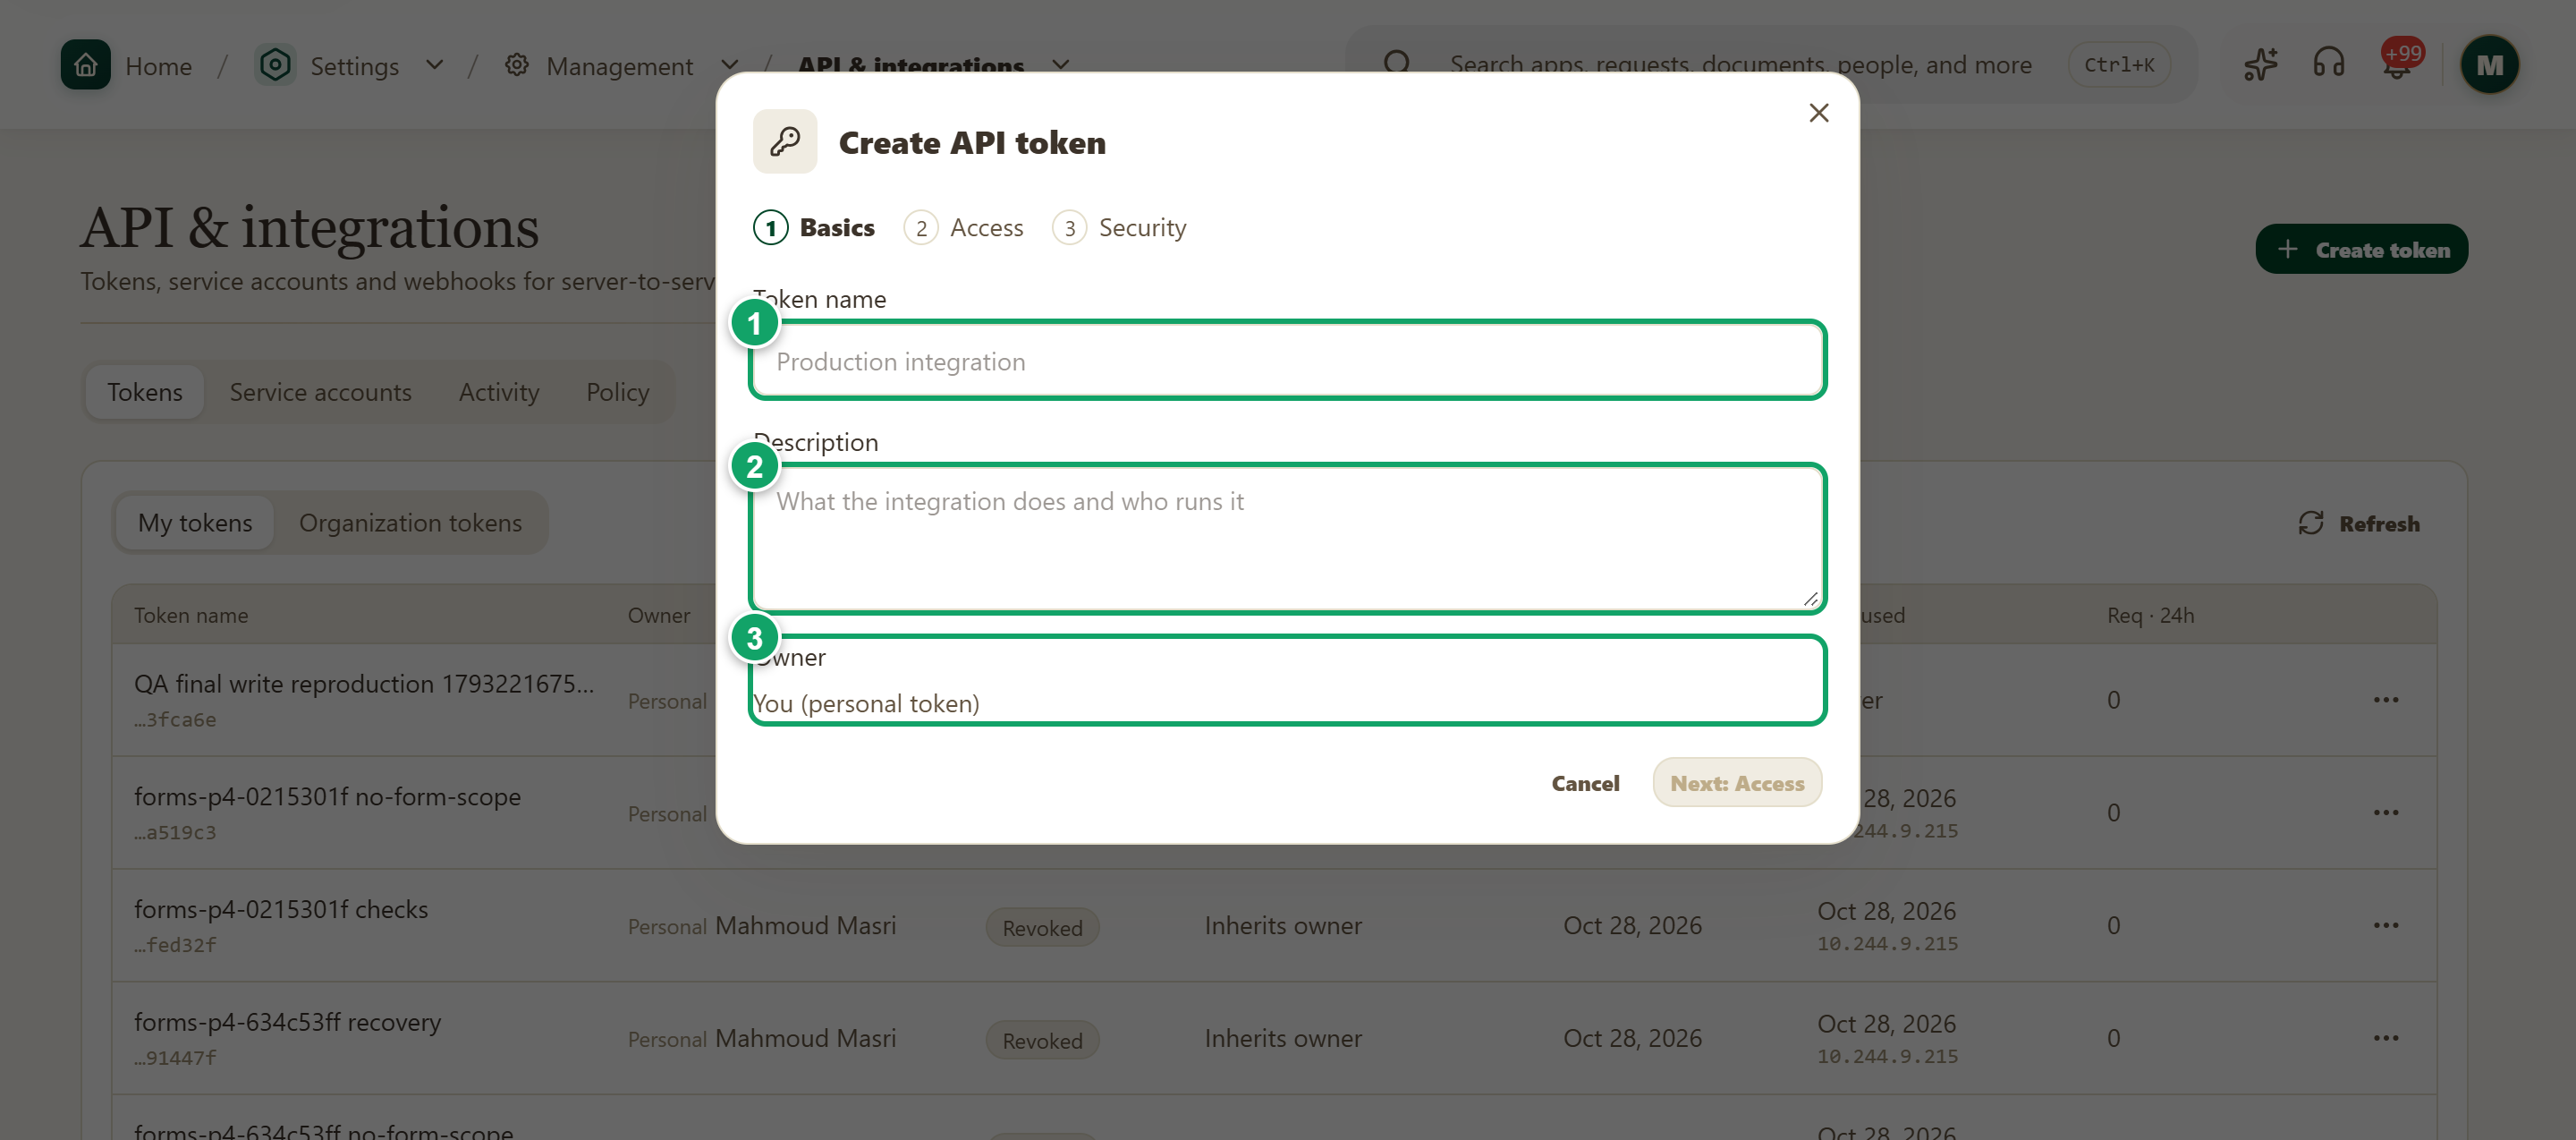
\includegraphics[width=0.95\linewidth,height=0.72\textheight,keepaspectratio]{figures/screens/ch08-api-create-en.png}
\caption{The Create token window: “Basics” step}
\label{fig:settings-api-create-screen}
\shotnote{Creating a token takes three steps: “Basics”, “Access” and “Security”. The window was opened to read and closed without creating a token. ① “Token name”: use a name that points to the system and purpose. ② “Description”. ③ “Owner”: you for a personal token, or a service account you manage.}
\end{figure}

\begin{table}[H]
\centering
\caption{What do you record when creating a token?}
\label{tab:settings-api-token-fields}
\begin{tabularx}{\linewidth}{R{4.2cm} Y}
\rcHeaderRow
\thh{Step} & \thh{What do you record?}\\
“Basics” & “Token name”, “Description” and “Owner”.\\
“Access” & “Everything the owner can do”, “Read-only”, or “Choose entities and actions”. A token never exceeds its owner’s permissions, and the last option is the narrowest.\\
“Security” & The expiry, within the limit the policy allows, and “IP allowlist” if you want to limit the token to certain networks.\\
\end{tabularx}
\end{table}

\begin{figure}[H]
\centering
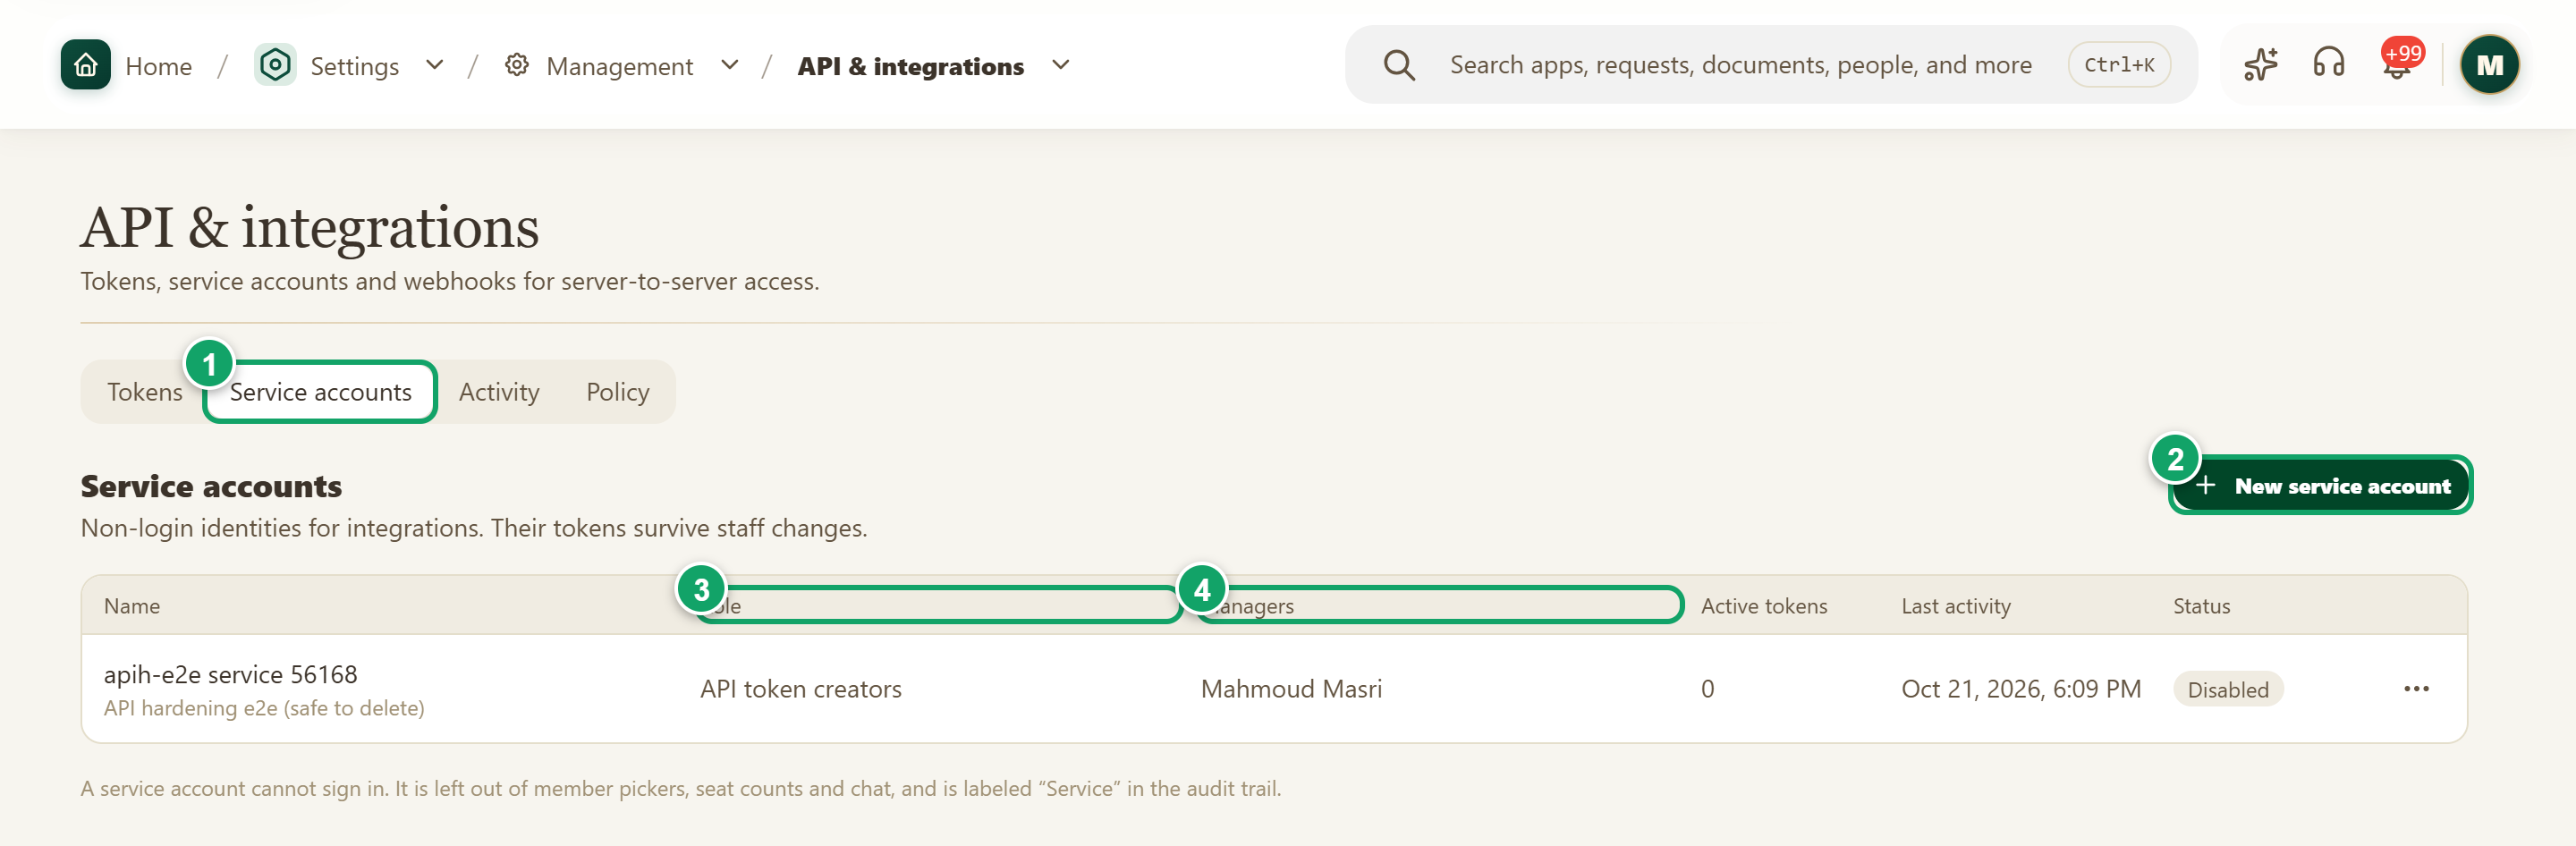
\includegraphics[width=0.95\linewidth,height=0.72\textheight,keepaspectratio]{figures/screens/ch08-api-service-accounts-en.png}
\caption{The “Service accounts” tab}
\label{fig:settings-api-service-accounts-screen}
\shotnote{A service account is an identity for one integration that never signs in, so its token does not stop when an employee leaves. It can do only what its role allows, and it stays out of member lists and seat counts. ① “Service accounts”. ② “New service account”. ③ “Role”. ④ “Managers”: who creates and replaces the account’s tokens and receives its alerts.}
\end{figure}

\begin{figure}[H]
\centering
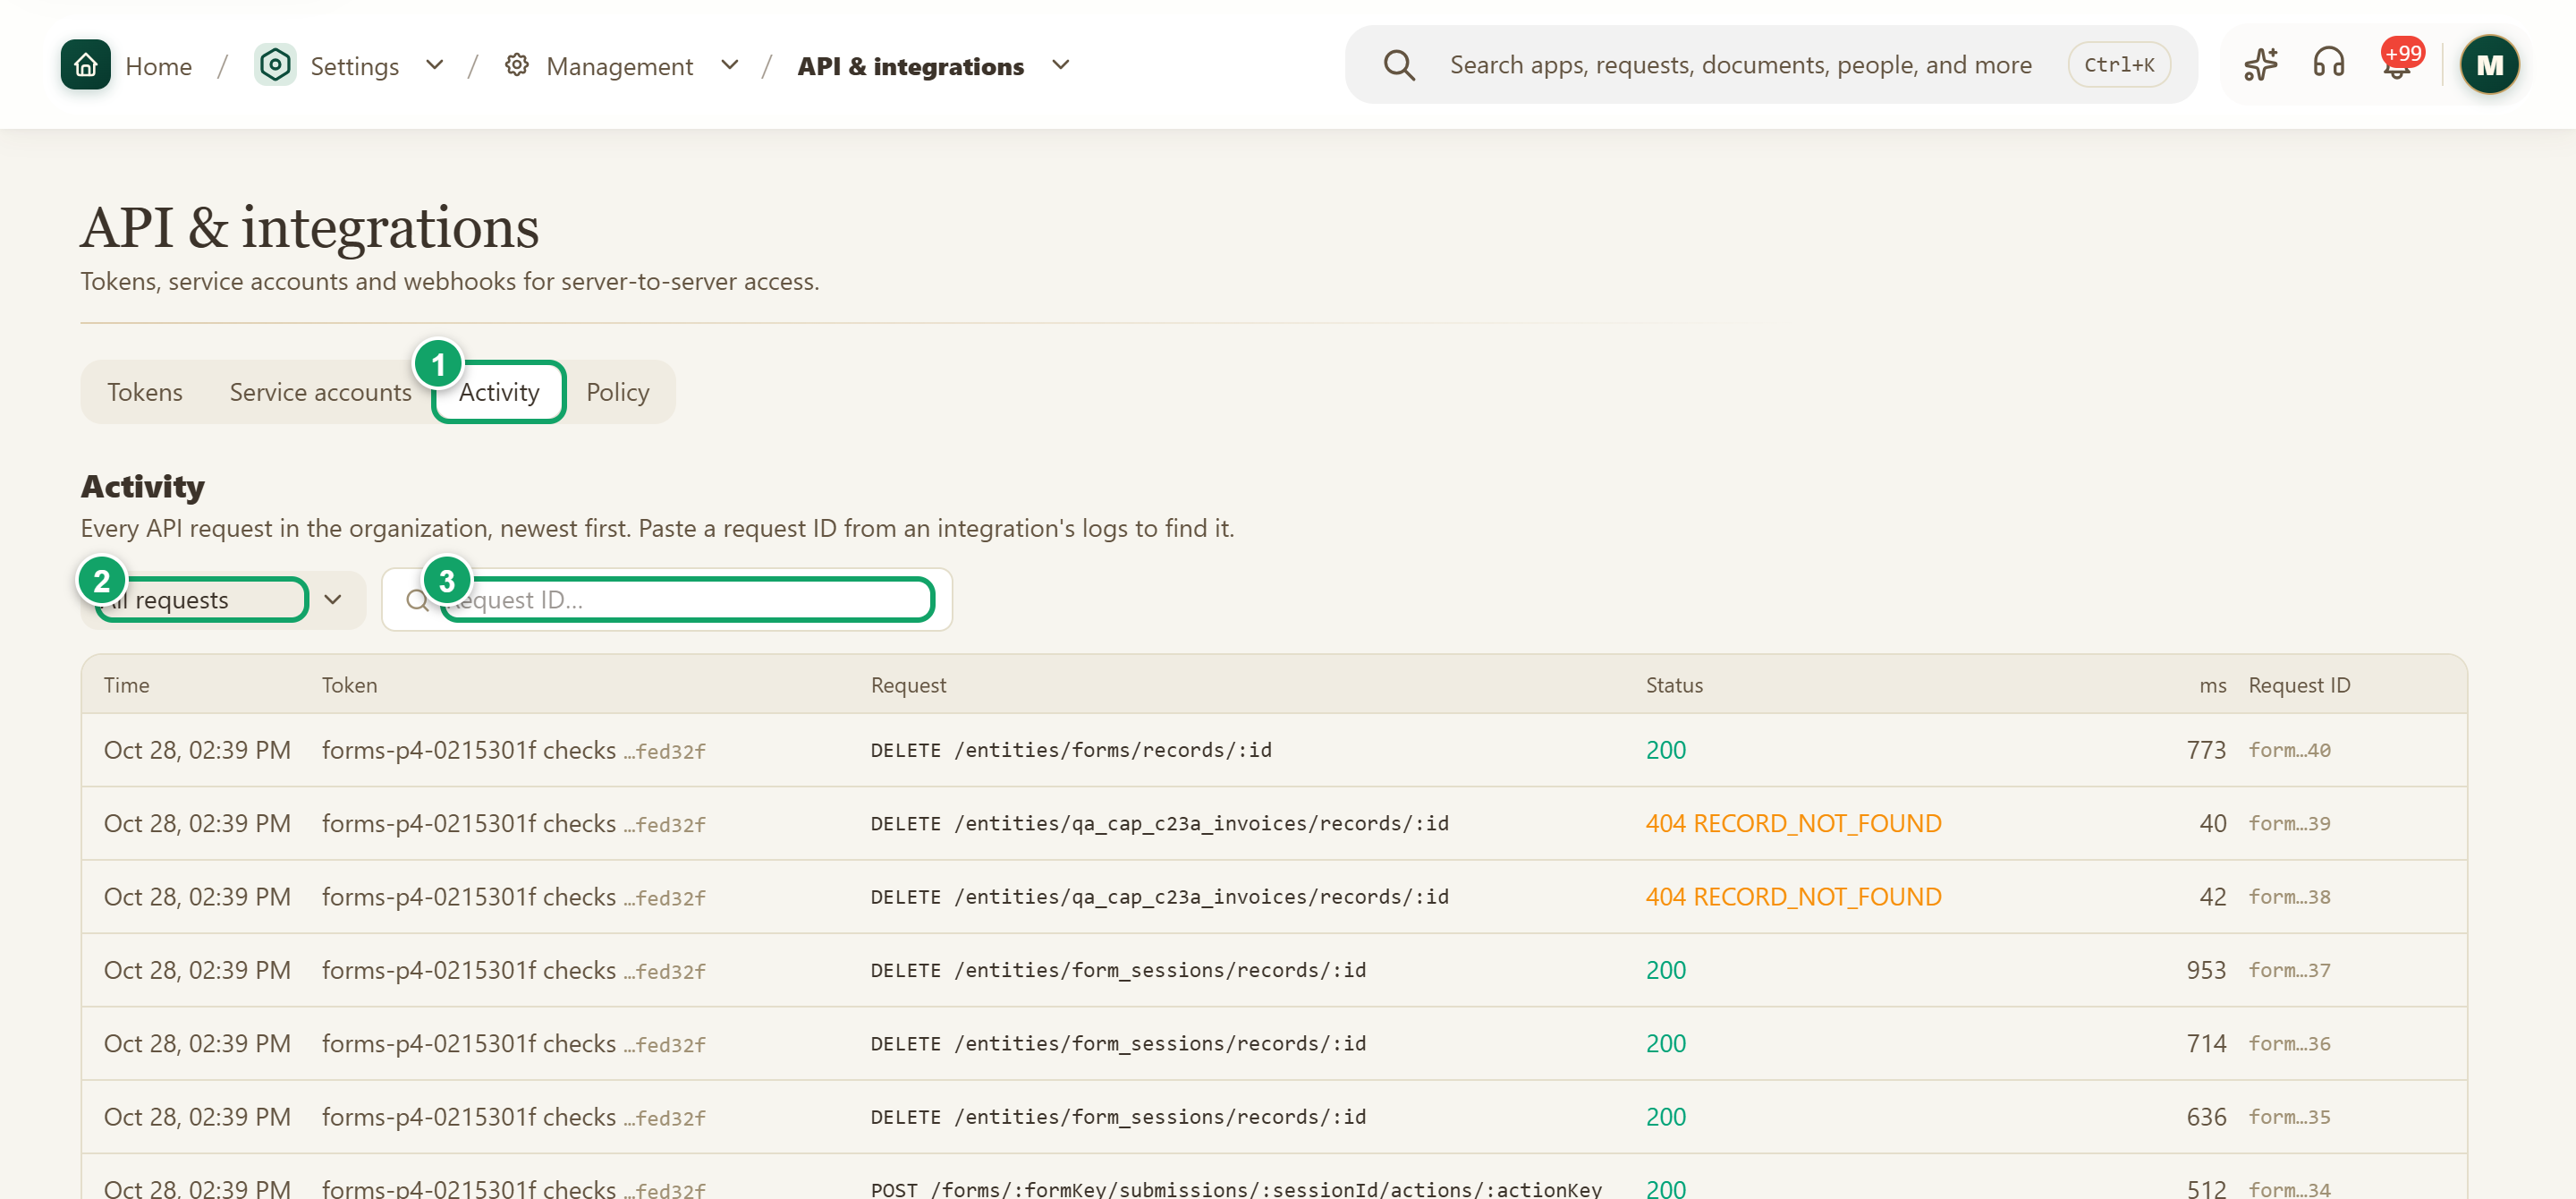
\includegraphics[width=0.95\linewidth,height=0.72\textheight,keepaspectratio]{figures/screens/ch08-api-activity-en.png}
\caption{The “Activity” tab}
\label{fig:settings-api-activity-screen}
\shotnote{This tab shows the API requests of the whole organization, newest first, and is where to start when an integration is reported broken. Request contents are not stored. ① “Activity”. ② The status filter: “All requests”, “Errors” or “Successful”. ③ “Request ID”: paste the ID from the integration’s logs to find one request.}
\end{figure}

\begin{figure}[H]
\centering
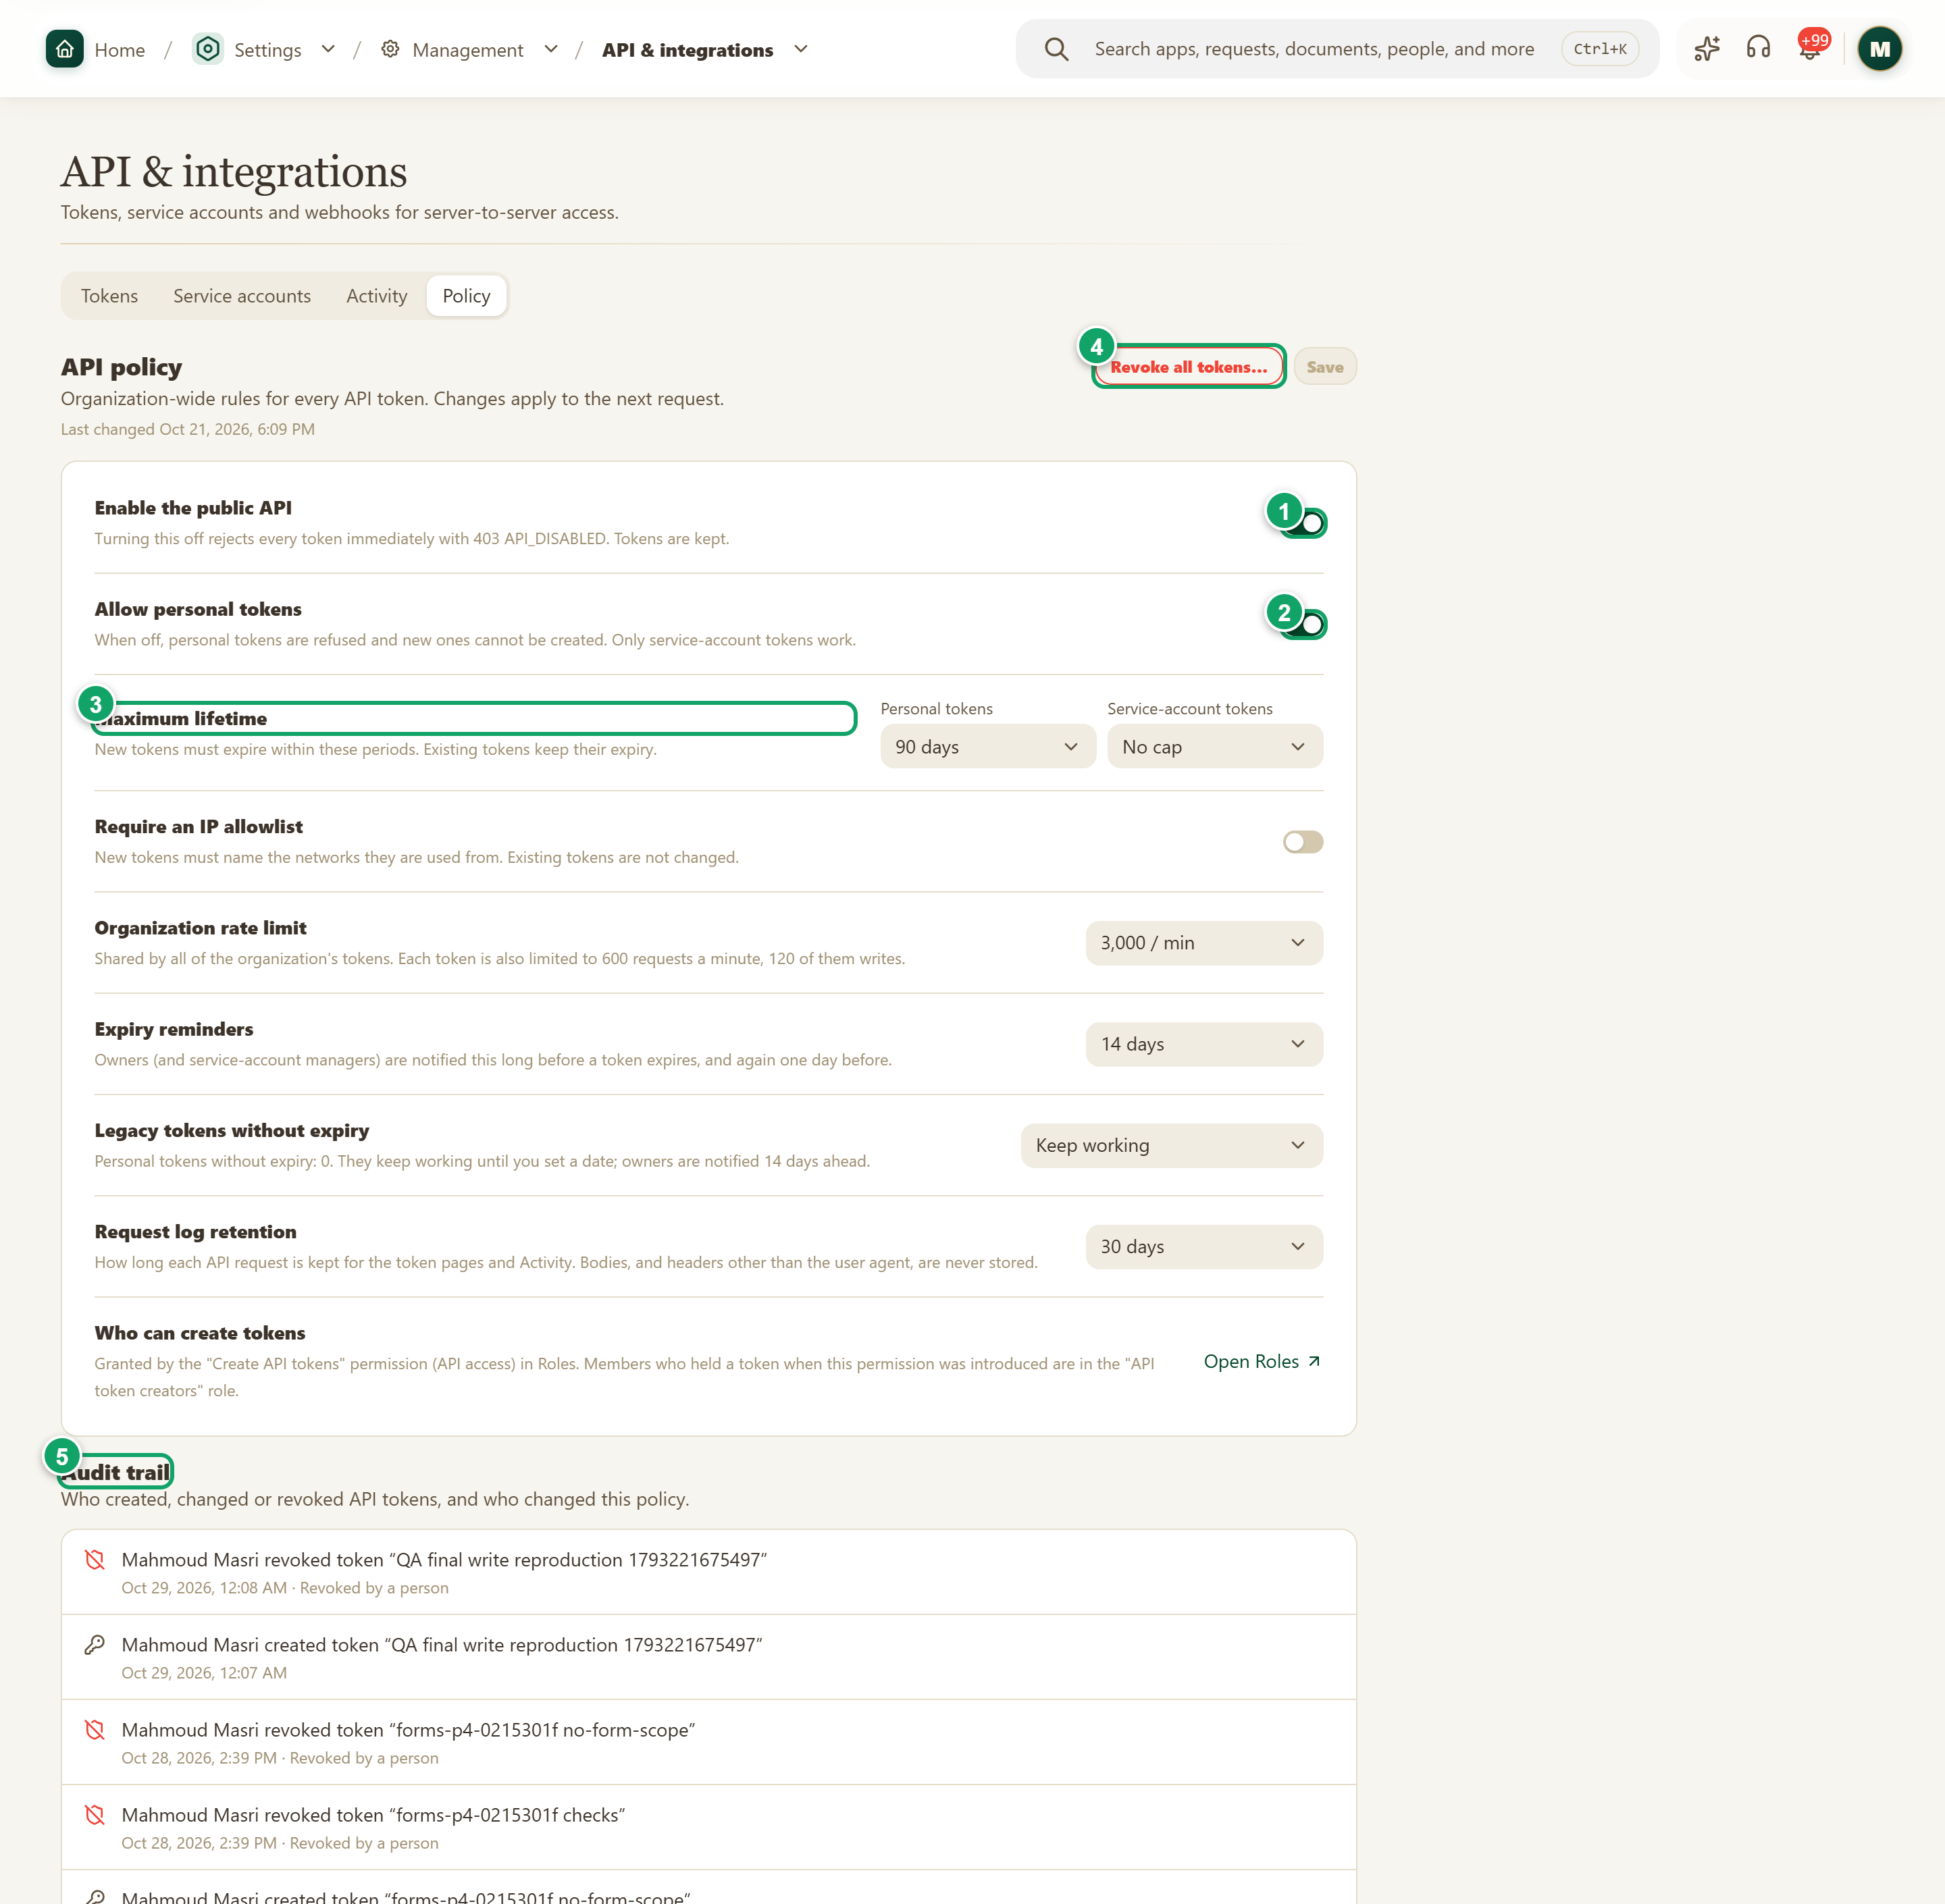
\includegraphics[width=0.95\linewidth,height=0.72\textheight,keepaspectratio]{figures/screens/ch08-api-policy-en.png}
\caption{The “Policy” tab and audit trail}
\label{fig:settings-api-policy-screen}
\shotnote{These rules apply to every token in the organization from the next request after saving, so change them with care: they can stop working integrations. The page was opened here to read only. ① “Enable the public API”: turning it off refuses every token at once, and the tokens are kept. ② “Allow personal tokens”. ③ “Maximum lifetime”: applies to new tokens. ④ “Revoke all tokens…”: an emergency action that cannot be undone. ⑤ “Audit trail”: who created, changed or revoked tokens, and who changed the policy.}
\end{figure}

\begin{table}[H]
\centering
\caption{What do you record in the API policy?}
\label{tab:settings-api-policy-fields}
\begin{tabularx}{\linewidth}{R{4.2cm} Y}
\rcHeaderRow
\thh{Field} & \thh{What do you record?}\\
“Enable the public API” & Stops every token when off; they work again when it is back on.\\
“Allow personal tokens” & When off, only service-account tokens work.\\
“Maximum lifetime” & A limit for “Personal tokens” and one for “Service-account tokens”. Existing tokens are not affected.\\
“Require an IP allowlist” & Makes every new token name the networks it is used from.\\
“Organization rate limit” & Requests a minute, shared by all the organization’s tokens.\\
“Expiry reminders” & How long before expiry owners are alerted, and again one day before.\\
“Legacy tokens without expiry” & Keep them working, or set a date when they stop.\\
“Request log retention” & How long requests stay on the token pages and in “Activity”.\\
“Who can create tokens” & A pointer to the “Create API tokens” permission in roles, with an “Open Roles” button.\\
\end{tabularx}
\end{table}

\begin{enumerate}
\item For a lasting integration, open “Service accounts”, press “New service account”, type the “Name”, choose the “Role” and “Managers”, then press “Create”.
\item Open “Tokens”, press “Create token”, and complete “Basics”, “Access” and “Security”. For a lasting integration, choose the service account as “Owner”.
\item Copy the token as soon as it appears to a safe place; it will not appear again. Then confirm you stored it and press “Done”.
\item To replace an old token, open its row menu, press “Rotate”, choose how long the old token keeps working, up to 7 days, then update the integration.
\item To stop a token, open its row menu and press “Revoke”. The token stops at once.
\item To change the rules, open “Policy”, change the value and press “Save”.
\end{enumerate}

\textbf{Check:} The token appears in the table as “Active”, “Last used” changes after the first request, and requests appear in “Activity” and on the token’s page. “Audit trail” records every token creation, revocation and policy change. If an integration stops, start from “Activity”, then check the token’s status and expiry, and that the API is still on.
